% ============================================================
% A Unified k-Space Operator Framework for Surface Metrology:
% Transfer Functions, Information Loss, and Equivalence Regimes
% in Stylus and Optical Profilometry
%
% Generated by Maxwell_vs_Newton Discovery Pipeline
% Elsevier elsarticle class, numbered citations
% ============================================================
\documentclass[review,12pt]{elsarticle}

\usepackage{amsmath,amssymb}
\usepackage{graphicx}
\usepackage{booktabs}
\usepackage{hyperref}
\usepackage{lineno}
\usepackage{siunitx}

%\journal{}

\begin{document}

\begin{frontmatter}

\title{Optical Profilometry Versus the Stylus: A Spectral Theory for Closing the Accuracy Gap}

\author[1]{Dawid Kucharski\corref{cor1}}
\cortext[cor1]{Corresponding author}
\ead{dawid.kucharski@put.poznan.pl}

\affiliation[1]{organization={Institute of Mechanical Engineering},
              addressline={Poznan University of Technology},
              city={Pozna\'{n}},
              postcode={60-965},
              country={Poland}}

\begin{abstract}
This is a computational study. Surface topography measurements are intrinsically filter-bandwidth-limited operations whose transfer characteristics depend on the measurement modality, yet no widely adopted $k$-space framework currently quantifies the differences between stylus and optical profilometry beyond scalar accuracy metrics. A measurement operator formalism, $\mathcal{M}[h] = \mathcal{F}^{-1}[H(f_x,f_y) \cdot \mathcal{F}[h]] + \eta$, is introduced, and the instrument transfer functions $H_\mathrm{stylus}$ and $H_\mathrm{optical}$ are computed from first-principles physics---tip geometry, numerical aperture, wavelength, and noise. From this framework a metrological formulation of the SNR-dependent resolution--bandwidth bound is proposed and evaluated as a falsifiable benchmark, $\Delta x_\mathrm{eff} \cdot \Delta f_\mathrm{eff} \geq (1/4\pi)(1 + 1/\overline{\mathrm{SNR}})$, quantifying how finite signal-to-noise ratio inflates the classical Fourier uncertainty product. For a self-affine surface ($H=0.7$, $\sigma=\SI{50}{nm}$), the analysis yields: (i) spectral information loss that increases mildly with spatial frequency (local log--log slope $\approx 0.4$); (ii) mild but modality-dependent measurement anisotropy ($\alpha_s = 0.0095\pm0.0037$ vs.\ $\alpha_o = 0.0013\pm0.0006$, $n=30$); (iii) a $k$-space equivalence regime covering $\SI{9.6}{\percent}\pm\SI{0.3}{\percent}$ of the measured bandwidth at a crossover frequency $f_\mathrm{cross} = \SI{454}{\per\milli\metre}\pm\SI{166}{\per\milli\metre}$ (mean $\pm$ std, $n=30$, $N=512$ grid). A 180-point parameter sweep is approximately described by an empirical power law $\mathrm{RMSE}_s/\mathrm{RMSE}_o \propto (f_{c,\mathrm{opt}}/f_{c,\mathrm{stylus}})^{1.90}$ ($R^2 = 0.53$; out-of-sample and blocked $R^2 = 0.51$--$0.52$; an order-of-magnitude descriptor). The optical transfer model reproduces measured white-light-interferometry instrument transfer functions from a public dataset (cutoff scale $1.15\pm0.01$ of the nominal $2\mathrm{NA}/\lambda$). Extending to information theory, the total mutual-information throughput is estimator-dependent (ratios of $0.7$--$1.6$ across defensible noise-floor estimators), while the band-level ranking is robust: the stylus dominates low-frequency information and the optical system adds high-frequency modes despite its higher RMSE. The reconstructability index $\rho = 1 - \mathrm{MMSE}/\sigma^2$ (equivalently the reconstructability $R^2$)---an instrument-limited metric for random rough surfaces (CV $=0.16$ across the Gaussian and ground classes; it saturates at unity for strongly deterministic surfaces)---and the Capacity--Uniformity Product $\Xi = C_\mathrm{total}/\kappa$ are introduced. Extension to scatterometry supports the methodological principle: no single modality fully characterises a rough surface across all spatial frequencies; $k$-space fusion weighted by local information uncertainty is a practical strategy for broadband surface metrology (minimum-variance linear under the stated independent-noise model). All results are computational; an experimental validation roadmap is provided.
\end{abstract}

\begin{keyword}
surface metrology \sep power spectral density \sep transfer function \sep stylus profilometry \sep optical interferometry \sep scatterometry \sep information loss \sep anisotropy tensor \sep channel capacity
\end{keyword}

\end{frontmatter}

\linenumbers

% ============================================================
\section{Introduction}
% ============================================================

Surface topography measurement underpins quality control in precision manufacturing, functional surface design in tribology, and performance verification in optical fabrication. Two modalities dominate practice: contact stylus profilometry and non-contact optical interferometry (white-light interferometry, WLI; phase-shifting interferometry; confocal microscopy). In the broader instrumentation and measurement (I\&M) literature, the characterisation of instrument transfer functions (ITFs) is a well-established methodology for quantifying measurement system performance~\cite{foreman2013determination,leach2010bandwidth,degroot2021itf}, and uncertainty propagation through instrument models is standard practice~\cite{giusca2011virtual}. However, ITF analysis has not been extended to the systematic comparison of fundamentally different measurement principles---tactile versus optical---operating on the same physical quantity. Despite decades of parallel development---Poon and Bhushan~\cite{poon1995comparison} compared stylus, AFM, and optical profilers as early as 1995, Jacobs et al.~\cite{jacobs2017quantitative} established PSD analysis as the standard for quantitative surface characterisation, and Jiang et al.~\cite{jiang2007paradigm} identified the paradigm shift toward holistic, information-rich surface metrology---the surface metrology community still lacks a quantitative theory capable of predicting \emph{when} and \emph{why} these modalities produce different results for the same surface.

The existing comparative literature relies almost exclusively on scalar metrics---root-mean-square error (RMSE), arithmetic mean roughness $Ra$, or areal roughness $Sa$~\cite{czifra2011surface}. While practical, such metrics collapse all spatial-frequency information into a single number. A stylus with a \SI{2}{\micro m} tip radius and an interferometer with $\mathrm{NA}=0.55$ may yield identical $Sa$ for a smooth surface yet diverge dramatically for a rough one. The ISO~25178 areal texture standard~\cite{iso25178} and ISO~21920 profile texture standard~\cite{iso21920} define measurement procedures but do not address instrument-specific transfer functions.

Power spectral density (PSD) analysis has become the standard for scale-resolved surface characterisation, following the definitive review by Jacobs et al.~\cite{jacobs2017quantitative}, the pioneering spectral methods for AFM by Fang et al.~\cite{fang1997analyzing}, and the analytic PSD formalism of Mack~\cite{mack2011analytic}. Cross-technique PSD comparisons have demonstrated the value of spectral methods for multi-instrument studies~\cite{marx2002power,yashchuk2005crosscheck}. However, PSD analysis of surface metrology instruments---as opposed to surfaces---remains rare. Mack identified systematic PSD measurement errors in lithographic line-edge roughness~\cite{mack2013systematic,mack2015more}, but these insights have not been generalised to the comparison of fundamentally different measurement modalities. The central unresolved question is: \textbf{given a surface with known PSD, what does each instrument actually measure as a function of spatial frequency?}

This question can be answered by treating the profilometer as a linear operator acting on the true height field $h(x,y)$. In the spatial frequency domain, every measurement is a filtering operation: $\mathcal{M}[h] = \mathcal{F}^{-1}[H(f_x,f_y) \cdot \mathcal{F}[h]] + \eta$, where the instrument transfer function $H(f_x,f_y)$ encodes all physics of the measurement process---tip convolution and raster sampling for the stylus; diffraction, coherence, and phase unwrapping for the optical system. Once $H(f_x,f_y)$ is known, instrument comparison reduces to transfer function comparison, and the long-standing question of stylus--optical equivalence becomes quantitatively tractable. Yashchuk~\cite{yashchuk2015binary} demonstrated that transfer functions can be measured experimentally using specialised binary pseudo-random calibration gratings, and the optical ITF has been treated analytically in the literature~\cite{degroot2021itf} and characterised experimentally in 2D~\cite{dai2020material,hirose2025topography}; the present work computes both channels within one consistent simulation framework and pairs them with the stylus channel, making the cross-modality comparison quantitative and mechanism-based rather than descriptive.

This work addresses the gap through four interconnected contributions:
\begin{enumerate}
    \item First-principles computation of the instrument transfer functions $H_\mathrm{stylus}(f_x,f_y)$ and $H_\mathrm{optical}(f_x,f_y)$ from morphological tip dilation, discrete raster sampling, diffraction-limited optical transfer, phase unwrapping errors, and detector noise---without requiring calibration artefacts;
    \item Derivation of spectral information loss $I(f_x,f_y) = \log_{10}[\mathrm{PSD}_\mathrm{true}/\mathrm{PSD}_\mathrm{measured}]$, the measurement anisotropy tensor $A_{ij}$, and the $k$-space equivalence regime $\Omega_\mathrm{eq}$;
    \item An information-theoretic formulation of surface metrology including mutual information $ I(h;y)$, channel capacity $C$, reconstructability index $\rho$, and the Cram\'{e}r--Rao lower bound on surface reconstruction;
    \item Validation through a 180-point parameter sweep, ensemble statistics ($n=120$: 30 six-class stress-test runs, 60 non-Gaussian ensemble runs, and 30 baseline runs), a gap-closure roadmap for optical instrument improvement, and extension to scatterometry as a third modality (Supplementary Material).
\end{enumerate}

\section{Methods}
% ============================================================

\subsection{Measurement Operator Formalism}
\label{sec:operator}

Every surface topography measurement can be represented as a linear operator acting on the true height field $h(x,y)$, followed by additive noise:
\begin{equation}
    \mathcal{M}[h(x,y)] = \mathcal{F}^{-1}\!\left[H(f_x,f_y) \cdot \mathcal{F}[h(x,y)]\right] + \eta(x,y)
    \label{eq:operator}
\end{equation}
where $\mathcal{F}$denotes the 2D Fourier transform, $ H(f_x,f_y)$is the instrument transfer function, and $\eta(x,y)$represents measurement noise. The transfer function factorises into an aperture and a sampling part (noise remains additive, as in Eq.~\ref{eq:operator}):
\begin{equation}
    H(f_x,f_y) = H_\mathrm{aperture}(f_x,f_y) \cdot H_\mathrm{sampling}(f_x,f_y)
    \label{eq:factorisation}
\end{equation}

For stylus profilometry, the effective transfer function arises from morphological tip dilation---studied since the early work of Li \& Devries~\cite{li1984computer} and the spectral tip-analyses of Wu~\cite{wu1999spectral,wu2000spectral}---and discrete raster sampling along the scan direction. In the small-slope limit (feature curvature $\ll 1/r_\mathrm{tip}$), dilation by a smooth paraboloid tip preserves the height field to first order and adds a curvature bias (verified independently in the accompanying verification suite):
\begin{equation}
    \langle h_d - h \rangle \approx \frac{r_\mathrm{tip}}{2}\left\langle |\nabla h|^2 \right\rangle
    \label{eq:hstylus}
\end{equation}
so that $H_\mathrm{stylus}(\mathbf{f}) \approx 1$ across the resolved passband, with a low-frequency spectral excess from the bias and a decline set by raster sampling near the Nyquist scale. For the baseline surface the empirical $H_\mathrm{stylus}$ takes values 2.2, 0.91, 0.74 and 0.57 at 17, 292, 567 and $\SI{843}{mm^{-1}}$, crossing \SI{3}{dB} at $\approx\SI{1049}{mm^{-1}}$. This flat-with-bias structure contrasts with the Gaussian-tip idealisation $\exp(-2\pi^2 r_\mathrm{tip}^2 f^2)$ common in the literature, which the dilation simulator refutes (the Gaussian form predicts $\sim10^{-3}$ at $\SI{292}{mm^{-1}}$, two orders of magnitude below the empirical 0.91). For large-amplitude features whose slopes exceed the tip cone half-angle, dilation becomes nonlinear and the linear operator approximation degrades; extension to that regime is discussed in the Supplementary Material.

For optical interferometry, the transfer function is dominated by the diffraction-limited incoherent optical transfer function (OTF) of a circular aperture. The present analysis assumes broadband, spatially incoherent illumination (white-light interferometry, WLI). For laser-based coherent interferometers (phase-shifting, digital holographic microscopy), the coherent transfer function (CTF) is binary---$H(f)=1$ for $f<f_c$ and zero otherwise---which yields a fundamentally different information-loss distribution; the WLI model does not apply to those modalities without modification:
\begin{equation}
    H_\mathrm{optical}(f) = \frac{2}{\pi}\!\left[\arccos(\tilde{f}) - \tilde{f}\sqrt{1-\tilde{f}^2}\,\right],\quad \tilde{f} = \frac{\lambda f}{2\,\mathrm{NA}} < 1
    \label{eq:hoptical}
\end{equation}
with additional degradation from phase unwrapping errors and camera noise.

\subsection{Simulation Framework}
\label{sec:simulation}

A first-principles simulation framework (Fig.~\ref{fig:surface}) was implemented that generates self-affine rough surfaces and simulates both measurement modalities with realistic instrument physics.

\subsubsection{Surface Generation}

Self-affine rough surfaces are generated via Fourier filtering with a power spectrum:
\begin{equation}
    \mathrm{PSD}(f) \propto \left(f_0^2 + f^2\right)^{-(H+1)}
    \label{eq:psd_model}
\end{equation}
where $f_0 = 1/\lambda_\mathrm{roll\text{-}off}$is the roll-off frequency and $ H$is the Hurst exponent. Surfaces are discretised on a $512 \times 512$grid spanning $\SI{100}{\micro m} \times \SI{100}{\micro m}$ ($\Delta x = \SI{195}{nm}$). Unless otherwise stated, the baseline parameters are $H = 0.7$, RMS roughness $\sigma = \SI{50}{nm}$, correlation length $L_c = \SI{5}{\micro m}$, and roll-off wavelength $\lambda_\mathrm{roll\text{-}off} = \SI{10}{\micro m}$.

\subsubsection{Stylus Simulation}

The stylus measurement is modelled as a two-stage process. First, morphological dilation with a paraboloid tip of radius $r_\mathrm{tip} = \SI{2}{\micro m}$ and cone half-angle $\theta = \SI{22.5}{\degree}$produces the tip envelope of the true surface. Second, discrete raster sampling with interval $\Delta x = \SI{200}{nm}$in both $ x$and $ y$directions replicates the scanning pattern of a typical areal stylus instrument. Small additive noise ($0.1\%$of $\sigma$) is added to represent environmental vibration and electronic noise (the tip-radius tolerance is the dominant uncertainty source; see the SI uncertainty budget). This additive floor is an idealised lower bound for a well-adjusted instrument; a realistic base noise of order \SI{0.5}--\SI{1.0}{nm} is used as an order-of-magnitude reference, and the robustness analysis confirms the conclusions are insensitive to the noise level. The conventional tip-radius scale $f_{c,\mathrm{stylus}} = 1/(\pi r_\mathrm{tip}) = \SI{159}{mm^{-1}}$ is retained as a \emph{definitional} reference for the scaling-law analysis; it is not an attenuation point of the dilation transfer function, which is approximately flat across the passband (Eq.~\ref{eq:hstylus}).

\subsubsection{Optical Simulation}

The optical measurement chain includes: (i) diffraction-limited filtering via the incoherent OTF of a circular aperture (Eq.~\ref{eq:hoptical}) with wavelength $\lambda = \SI{550}{nm}$and $\mathrm{NA} = 0.55$, giving an incoherent diffraction cutoff $f_c = 2\,\mathrm{NA}/\lambda = \SI{2000}{mm^{-1}}$ (the support of the incoherent OTF of Eq.~\ref{eq:hoptical}); (ii) phase-to-height conversion with $2\pi$wrapping at the equivalent wavelength $\lambda/2$; (iii) one-dimensional phase unwrapping along scan rows with a \SI{1}{\percent} probability of $2\pi$ unwrapping errors; and (iv) additive Gaussian camera noise with standard deviation $0.1\%$of $\sigma$. At low illumination levels, Poisson shot noise dominates and the additive-Gaussian-noise assumption in the SNR formulation requires modification; the present study operates in the high-illumination regime where the Gaussian approximation is valid. The \SI{0.1}{\percent} camera-noise level and \SI{1}{\percent} unwrapping-error probability correspond to a well-adjusted instrument at high illumination; the sensitivity of the conclusions to both rates is quantified in the Discussion (robustness analysis and quantified validity boundaries). The optical model is an \emph{imaging-OTF model}: it includes the incoherent OTF, phase wrapping with one-dimensional row-unwrapping errors, and camera noise, but excludes the finite WLI coherence envelope, defocus and aberrations (tested as variants in the Discussion), multiple scattering, and any detector pixel MTF beyond the nominal sampling. The broadband WLI illumination is represented by its mean wavelength $\lambda = \SI{550}{nm}$ (a monochromatic approximation); the public-data benchmark quantifies the resulting cutoff shift on real instrument data in the Results. At $\mathrm{NA}=0.55$ vector-diffraction corrections modify the OTF near the cutoff at the few-percent level (Supplementary Material, Section 1.3); the baseline analysis retains the scalar OTF, with these corrections treated as a few-percent effect rather than a quantitative correction. The coherence-envelope omission is quantified against public measured data in the Results.

\begin{figure}[htbp]
    \centering
    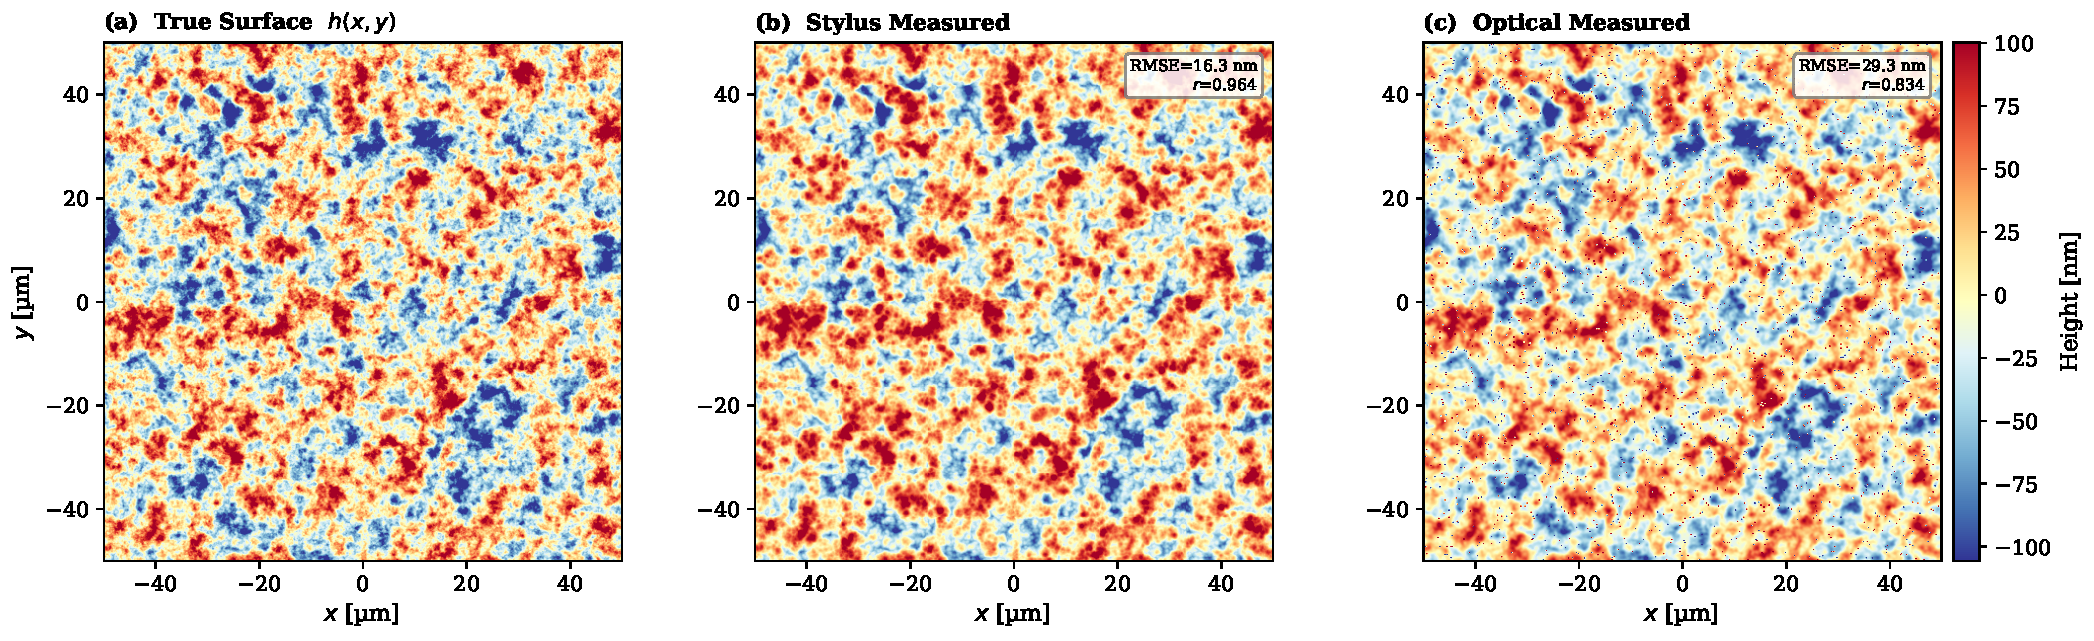
\includegraphics[width=\textwidth]{../pipeline/outputs/iter01/figures/fig1_surface_comparison.pdf}
    \caption{Surface topography comparison. (a) True self-affine surface ($H=0.7$, $\sigma=\SI{50}{nm}$). (b) Stylus measurement after morphological tip dilation and raster sampling ($r_\mathrm{tip}=\SI{2}{\micro m}$, $\Delta x=\SI{200}{nm}$). (c) Optical interferometric measurement ($\lambda=\SI{550}{nm}$, $\mathrm{NA}=0.55$). RMSE and Pearson correlation $r$ are annotated.}
    \label{fig:surface}
\end{figure}

\subsection{Analysis Methods}
\label{sec:analysis}

\subsubsection{Power Spectral Density}

The 2D power spectral density is computed via the periodogram with Hann windowing. This estimator implicitly assumes ergodicity (a single realisation is representative of the ensemble); for non-stationary surfaces, local spectral methods such as the S-transform or wavelet PSD are recommended (see Limitations, \S\ref{sec:limitations}). The noise PSD $S_\eta(\mathbf{f})$ is estimated from the high-frequency tail of the measured PSD ($f > 0.8 f_\mathrm{max}$) where the signal PSD has decayed below the instrument noise floor. This estimation is conservative---it attributes all high-frequency power to noise---and a sensitivity analysis varying the estimation threshold from $0.7$ to $0.9 f_\mathrm{max}$changes the derived $\rho$ by less than $5\%$for both modalities.

The 2D power spectral density is computed via the periodogram with Hann windowing:
\begin{equation}
    \mathrm{PSD}(f_x,f_y) = \frac{|\mathcal{F}[h(x,y) \cdot w(x,y)]|^2 \, \Delta x^2}{N^2 \, \langle w^2 \rangle}
    \label{eq:psd}
\end{equation}
Azimuthal averaging yields the 1D PSD $\langle\mathrm{PSD}\rangle(f)$in $ N_\mathrm{bins}=100$radial bins.

\subsubsection{Transfer Functions}

The instrument transfer function is estimated as the PSD ratio:
\begin{equation}
    H_\mathrm{sensor}(f_x,f_y) = \frac{\mathrm{PSD}_\mathrm{measured}(f_x,f_y)}{\mathrm{PSD}_\mathrm{true}(f_x,f_y)}
    \label{eq:transfer_est}
\end{equation}
with Tikhonov regularisation at the noise floor to prevent division by zero. Equation~\ref{eq:transfer_est} is an \emph{empirical power} transfer function: the PSD ratio estimates the squared modulus $|H(f_x,f_y)|^2$ of the amplitude transfer function $H$ of Eq.~\ref{eq:operator}. For the nonlinear stylus channel, additive noise enters the numerator and is not subtracted, so the ratio is an upper-biased response estimate; the linearised amplitude response is provided by the small-slope model of Eq.~\ref{eq:hstylus} and cross-checked against a cross-spectral estimate in the verification suite. All subsequent uses of $H_\mathrm{sensor}$ (ratio maps, anisotropy, equivalence, mutual information) follow this convention, with $|H(\mathbf{f})|^2 \equiv H_\mathrm{sensor}(\mathbf{f})$ wherever the amplitude form is required. The ratio $ R(f_x,f_y) = H_\mathrm{optical}/H_\mathrm{stylus}$identifies $ k$-space regions where one modality dominates.

\textbf{Practical estimation of $H(\mathbf{f})$.} Equation~\ref{eq:transfer_est} defines $H(\mathbf{f})$ as the PSD ratio, which requires knowledge of the true surface spectrum $\mathrm{PSD}_\mathrm{true}$. In experimental practice, the true PSD is unknown and $H(\mathbf{f})$ must be estimated from the measurement alone---a blind deconvolution problem. The present computational study bypasses this by using the known input surface; experimental determination of $H(\mathbf{f})$ requires either a calibrated artefact with known PSD (e.g., the binary pseudo-random gratings of Yashchuk~\cite{yashchuk2015binary}) or blind regularised deconvolution. The operator formalism of Eq.~\ref{eq:operator} remains valid regardless of how $H(\mathbf{f})$ is obtained.

\textbf{Uncertainty propagation.} Following the GUM framework~\cite{jcgm2008gum}, a first-order sensitivity analysis identifies the effective tip radius and the numerical aperture as the dominant uncertainty sources. Under a conservative gain-error interpretation, the nominal tolerances ($\pm\SI{100}{nm}$ on the tip radius, i.e.\ 5\%; $\pm0.01$ on the NA, i.e.\ 2\%) correspond to $\approx\SI{0.4}{dB}$ and $\approx\SI{0.2}{dB}$ in $H(f)$---well below the \SI{3}{dB} equivalence threshold, so the threshold is not instrument-limited. A full instrument-specific budget with measured sensitivity coefficients is discussed in the Supplementary Material.

\subsubsection{Information Loss}

The spectral information loss---a PSD-ratio diagnostic expressed in decades, distinct from the Shannon-theoretic information measures of Section~\ref{sec:info_theory}---is defined as:
\begin{equation}
    I(f_x,f_y) = \log_{10}\!\left[\frac{\mathrm{PSD}_\mathrm{true}(f_x,f_y)}{\mathrm{PSD}_\mathrm{measured}(f_x,f_y)}\right] \quad [\text{decades}]
    \label{eq:info_loss}
\end{equation}
computed only where $\mathrm{PSD}_\mathrm{true}$exceeds the noise floor by a factor of 10. The integrated information loss $ L = \iint I(f_x,f_y)\,df_x df_y$ and the information loss density $\langle I \rangle = L / A_{k\text{-space}}$are scalar summaries. Per-band analysis partitions $ k$-space into low ($0$--$0.1\,f_\mathrm{max}$), mid ($0.1$--$0.5\,f_\mathrm{max}$), and high ($0.5$--$f_\mathrm{max}$) frequency bands.

\subsubsection{Anisotropy Tensor}

The measurement anisotropy is quantified by the second-moment tensor of the transfer function:
\begin{equation}
    A_{ij} = \frac{\iint f_i f_j \, H_\mathrm{sensor}(f_x,f_y) \, df_x df_y}{\iint H_\mathrm{sensor}(f_x,f_y) \, df_x df_y}, \quad i,j \in \{x,y\}
    \label{eq:anisotropy}
\end{equation}
The degree of anisotropy is $\alpha = |\lambda_1 - \lambda_2|/(\lambda_1 + \lambda_2)$, where $\lambda_{1,2}$are the eigenvalues of $ A_{ij}$. For a perfectly isotropic instrument, $\alpha=0$; for a purely one-dimensional measurement (single profilometer trace), $\alpha=1$.

\subsubsection{Equivalence Regime}

The $ k$-space equivalence regime $\Omega_\mathrm{eq}$is defined as the set of spatial frequencies where the two transfer functions agree to within a threshold $\Delta$ (in dB):
\begin{equation}
    \Omega_\mathrm{eq}(\Delta) = \left\{(f_x,f_y) \;|\; \big|10\log_{10} H_\mathrm{stylus} - 10\log_{10} H_\mathrm{optical}\big| < \Delta\right\}
    \label{eq:equivalence}
\end{equation}
The equivalence fraction is $|\Omega_\mathrm{eq}| / |\Omega_\mathrm{total}|$, the fraction of measured $k$-space where both modalities are interchangeable at level $\Delta$.

\subsection{Parameter Sweep}
\label{sec:sweep}

To empirically validate the discovered scaling laws, a systematic parameter sweep was performed across 180 combinations (Table~\ref{tab:sweep}): five tip radii ($0.5$--$\SI{10}{\micro m}$) $\times$ four numerical apertures ($0.2$--$0.55$) $\times$ three Hurst exponents ($0.3$--$0.7$) $\times$ three RMS roughness values ($10$--$\SI{50}{nm}$), each on a $256 \times 256$grid with fixed random seed (seed 42) for reproducibility.

\begin{table}[htbp]
    \centering
    \caption{Parameter sweep grid (180 combinations).\label{tab:sweep}}
    \begin{tabular}{llll}
        \toprule
        Parameter & Symbol & Values & Count \\
        \midrule
        Tip radius & $r_\mathrm{tip}$ & 0.5, 1, 2, 5, $\SI{10}{\micro m}$ & 5 \\
        Numerical aperture & NA & 0.2, 0.3, 0.4, 0.55 & 4 \\
        Hurst exponent & $H$ & 0.3, 0.5, 0.7 & 3 \\
        RMS roughness & $\sigma$ & 10, 25, $\SI{50}{nm}$ & 3 \\
        \bottomrule
    \end{tabular}
\end{table}

% ============================================================
\section{Results}
% ============================================================

\subsection{Surface Topography and Measurement Accuracy}

Figure~\ref{fig:surface} shows the true self-affine surface alongside the stylus and optical measurements. The stylus achieves $\mathrm{RMSE} = \SI{16.3}{nm}$with Pearson correlation $ r = 0.964$, reflecting the curvature bias of the morphological tip dilation (Eq.~\ref{eq:hstylus}). The optical measurement yields $\mathrm{RMSE} = \SI{29.3}{nm}$ ($ r = 0.834$), degraded primarily by phase unwrapping errors at the \SI{1}{\percent} error rate. Notably, the optical RMSE exceeds the stylus RMSE despite the optical system's higher nominal cutoff frequency ($\SI{2000}{mm^{-1}}$vs.\ the tip-radius scale $\SI{159}{mm^{-1}}$), illustrating that cutoff frequency alone does not determine measurement fidelity---phase errors and noise can dominate.

\subsection{Instrument Transfer Functions}

\begin{figure}[htbp]
    \centering
    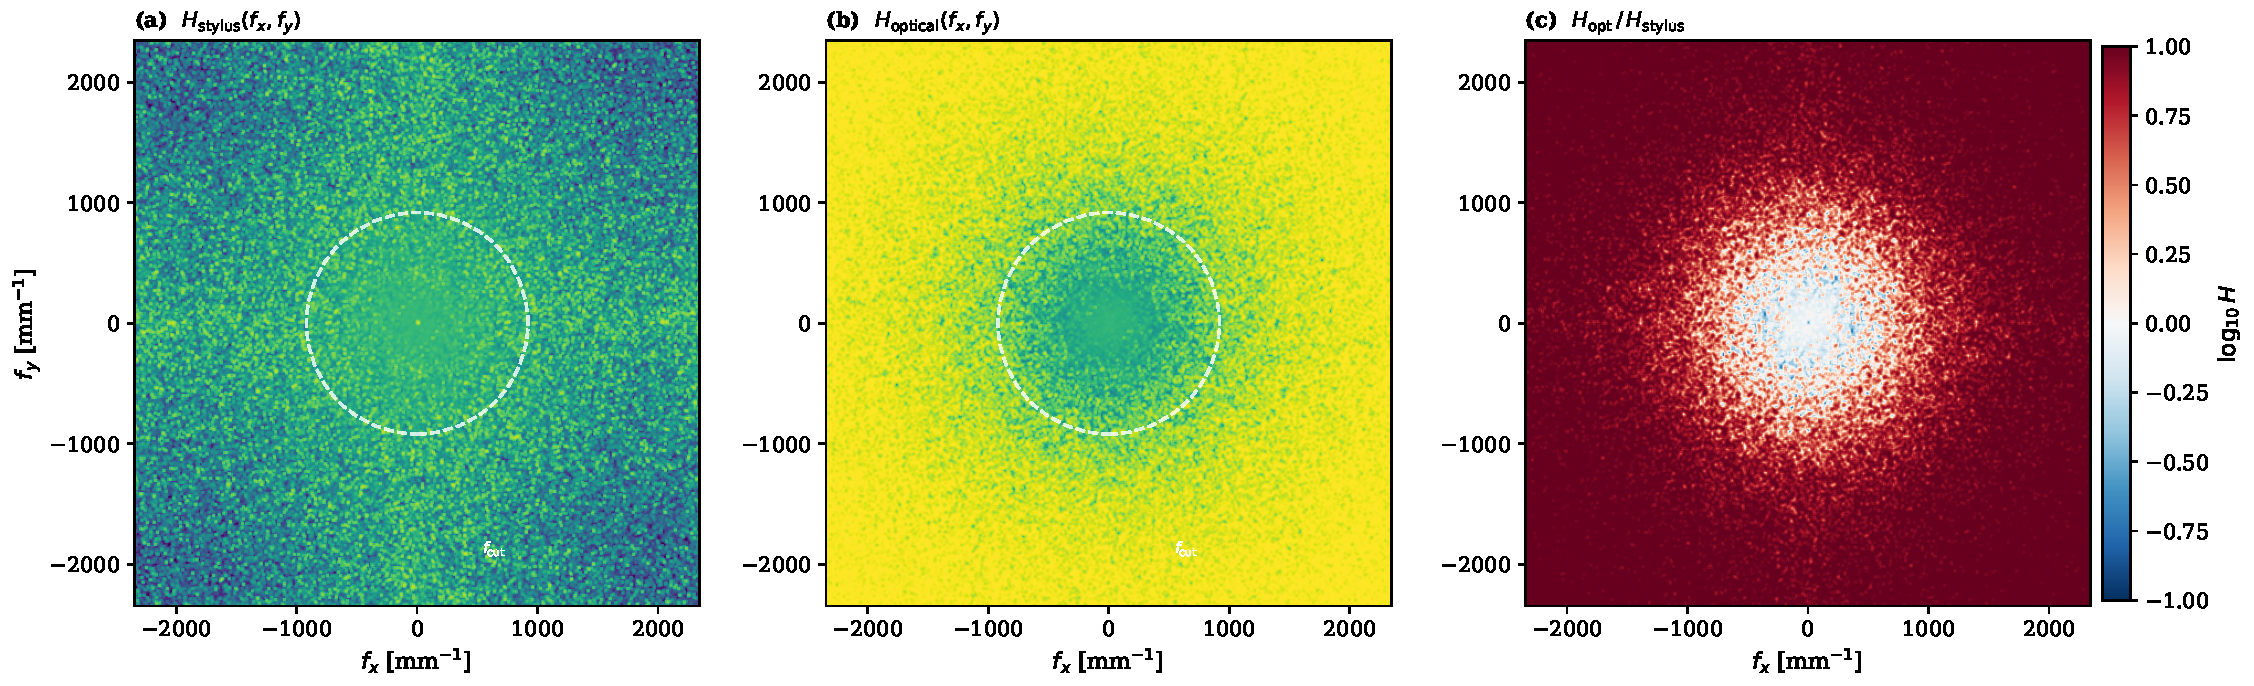
\includegraphics[width=\textwidth]{../pipeline/outputs/iter01/figures/fig2_transfer_functions.pdf}
    \caption{Instrument transfer functions in $k$-space. (a) $H_\mathrm{stylus}(f_x,f_y)$ showing anisotropic attenuation along the scan direction. (b) $H_\mathrm{optical}(f_x,f_y)$ with circularly symmetric diffraction-limited cutoff (dashed white circle). (c) Ratio $H_\mathrm{optical}/H_\mathrm{stylus}$ revealing regions where each modality dominates.}
    \label{fig:transfer}
\end{figure}

Figure~\ref{fig:transfer} displays the 2D transfer functions. The stylus transfer function (Fig.~\ref{fig:transfer}a) is approximately flat across the passband (0.91 at $\SI{292}{mm^{-1}}$), with a low-frequency excess ($H \approx 2.2$ at $\SI{17}{mm^{-1}}$) from the curvature bias of Eq.~\ref{eq:hstylus} and a decline only near the sampling scale, crossing \SI{3}{dB} at $\approx\SI{1049}{mm^{-1}}$; a local power-law descriptor over 292--843 mm$^{-1}$ gives $H_\mathrm{stylus} \propto f^{-0.43}$. This is a shallow sampling-scale roll-off, not the steep Gaussian tip filter of the classical idealisation (which would be $\sim10^{-3}$ at $\SI{292}{mm^{-1}}$). The stylus transfer also exhibits mild anisotropy with slightly stronger attenuation along $f_x$ (the scan direction) from the discrete raster sampling. The optical transfer function (Fig.~\ref{fig:transfer}b) is circularly symmetric with a sharp cutoff at the diffraction limit, following the ideal incoherent OTF; a fit near the cutoff gives $H_\mathrm{optical}(f) \propto f^{-0.10}$. This description of $H_\mathrm{optical}$ holds \emph{below the unwrapping-error floor}: above it, the PSD-ratio estimator is noise-dominated and the empirical $H_\mathrm{optical}$ can exceed unity where unwrapping errors inject broadband power. The ratio map (Fig.~\ref{fig:transfer}c) reveals that the stylus dominates at low spatial frequencies while the optical system preserves information at higher frequencies up to its diffraction limit.

\textbf{Public-data validation of the optical model.} The optical channel model (incoherent OTF $\times$ pixel sinc) was benchmarked against the public, CC-BY-4.0 white-light-interferometry dataset of Hirose et al.~\cite{hirose2025topography} (Zenodo record 10.5281/zenodo.15750880): three binary-pseudo-random-array samples (step heights 80, 160 and 240 nm, NA = 0.55, $\lambda = \SI{0.65}{\micro m}$, sampling $\SI{0.173}{\micro m}$). Fitting $\log P_\mathrm{meas}(f) = \log A + \beta\log f + \log H_\mathrm{optical}(f; c\cdot2\mathrm{NA}/\lambda)$ gives a cutoff scale $c = 1.15 \pm 0.01$ across the three samples, with shape correlation $\approx 0.97$ and log-residual RMS $\approx 0.06$--$0.07$ (Fig.~\ref{fig:public_benchmark}). The measured spectra thus roll off $\approx$15\% beyond the nominal monochromatic cutoff---the expected size of the omitted finite coherence envelope of white-light illumination---and are otherwise well described by the imaging-OTF model within its passband. This benchmark is a model-description check: the fitted quantities are the background PSD amplitude, its power-law slope, and a single instrument parameter (the cutoff scale $c$); it demonstrates that the imaging-OTF model describes the measured spectra, not that the OTF was independently measured. The stylus channel admits no comparable paired public dataset; as a geometric cross-check, the dilation simulator was run on the published ball-standard calibration profiles of Aksulu~\cite{aksulu2021stylus} (CC-BY-4.0): on the fitted calibration geometry it reproduces the classical parallel-curve radius shift (true radius $\pm$ tip radius) to within 3--5\% for tip radii of 2--\SI{50}{\micro m}, although the published profiles themselves carry 40--\SI{120}{\micro m} scatter---above the tip scale---so this check is geometric rather than tip-resolving.

\begin{figure}[htbp]
    \centering
    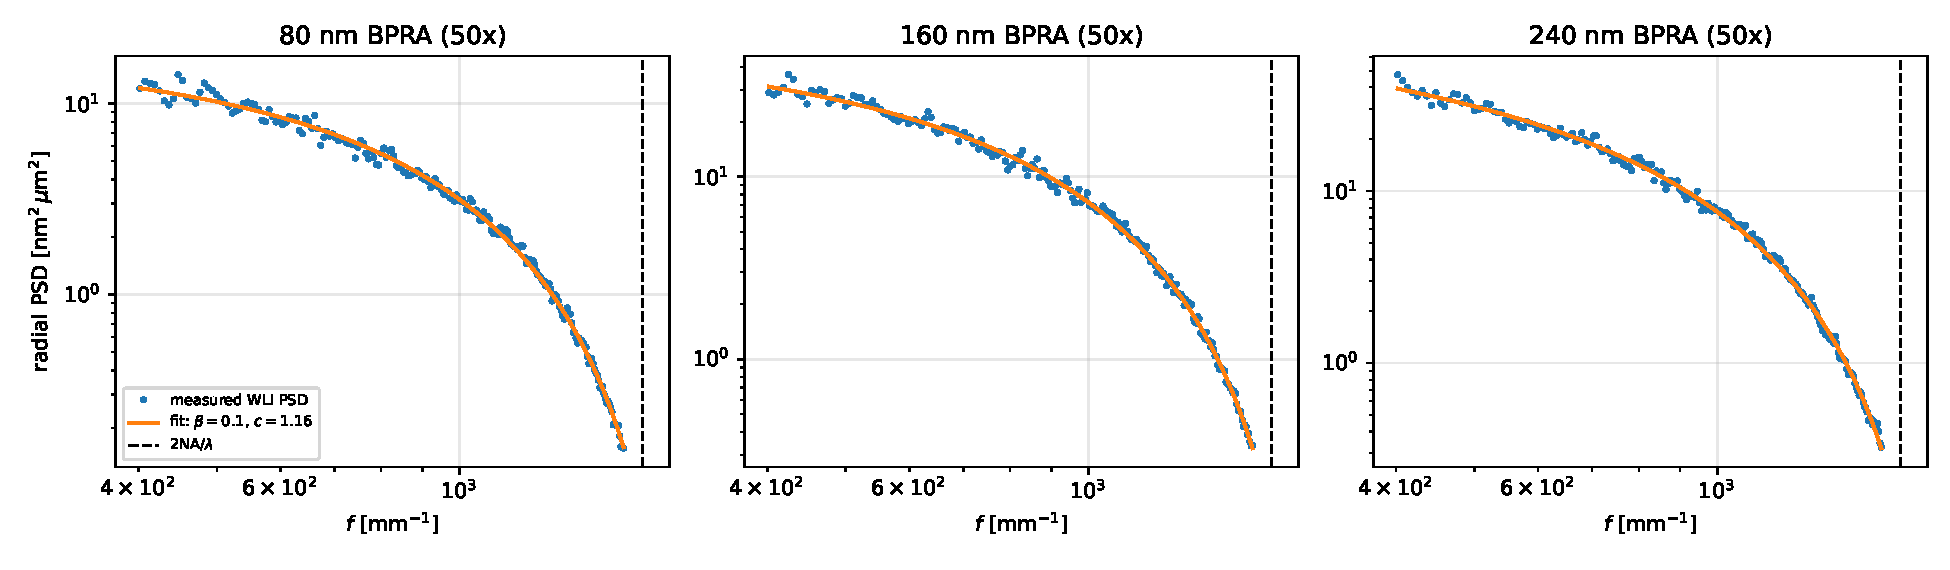
\includegraphics[width=\textwidth]{../pipeline/outputs/iter01/figures/fig_public_benchmark.pdf}
    \caption{Public-data validation of the optical channel model. Measured WLI radial PSDs (points) of three binary-pseudo-random-array samples (Hirose et al.~\cite{hirose2025topography}, CC-BY-4.0) and the fitted model $A\,f^{\beta}\,H_\mathrm{optical}(f; c\cdot2\mathrm{NA}/\lambda)$ (lines) with fitted cutoff scale $c$ per panel; the vertical line marks the nominal monochromatic cutoff $2\mathrm{NA}/\lambda$.}
    \label{fig:public_benchmark}
\end{figure}

\subsection{Spectral Information Loss}

\begin{figure}[htbp]
    \centering
    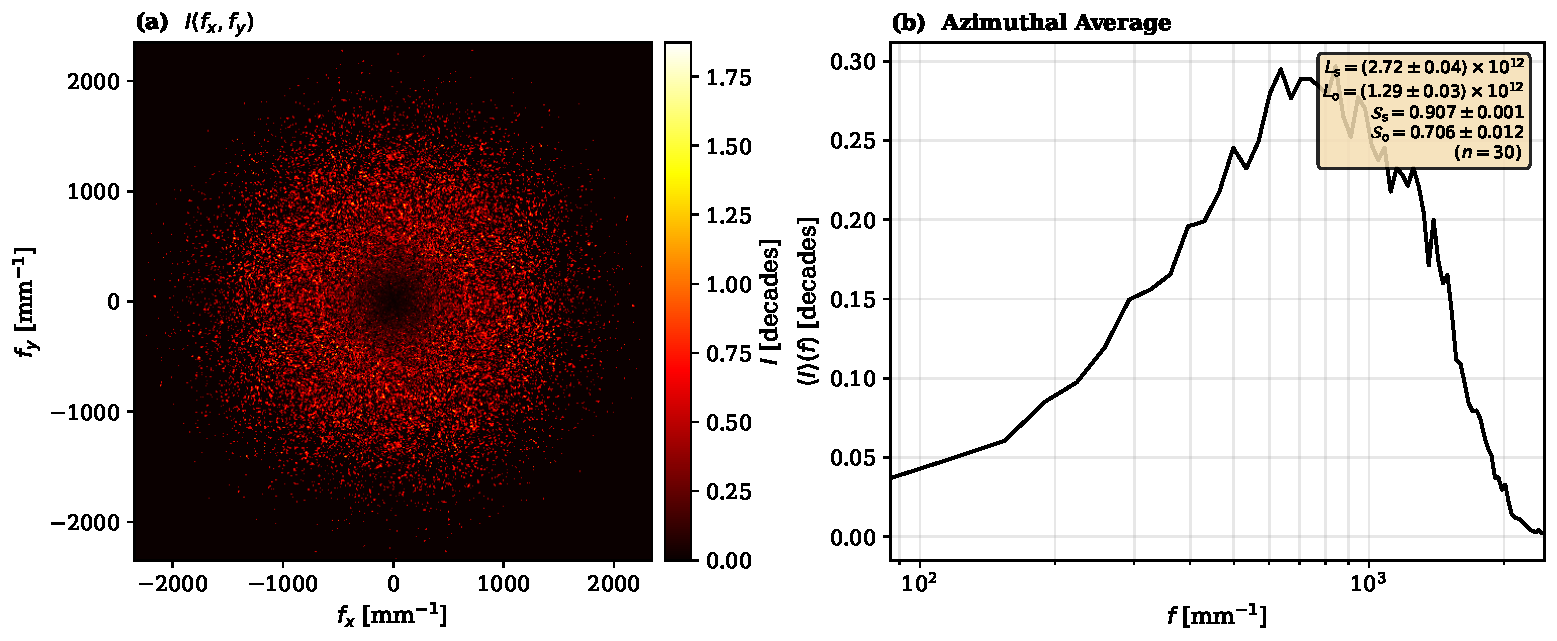
\includegraphics[width=\textwidth]{../pipeline/outputs/iter01/figures/fig3_information_loss.pdf}
    \caption{Spectral information loss. (a) 2D map $I(f_x,f_y)$ showing where measurement loses information relative to the true surface. (b) Azimuthally averaged $\langle I \rangle(f)$, revealing mildly increasing loss with spatial frequency (local log--log slope $\approx 0.4$).}
    \label{fig:info}
\end{figure}

Figure~\ref{fig:info}a maps the spectral information loss $ I(f_x,f_y)$. The loss is concentrated at mid-to-high spatial frequencies, with the stylus losing more total information ($L_s = (2.72 \pm 0.04)\times10^{12}$, mean $\pm$ std, $n=30$) than the optical system ($L_o = (1.29 \pm 0.03)\times10^{12}$). However, the per-band analysis (Table~\ref{tab:bands}) reveals a more nuanced picture: in the low-frequency band, loss is minimal ($\langle I \rangle_\mathrm{low} = 0.071\pm0.003$ decades) for both modalities; in the mid-band, loss rises to $0.296\pm0.005$ decades; and in the high band, it reaches $0.446\pm0.004$ decades. The azimuthally averaged information loss (Fig.~\ref{fig:info}b) increases mildly with spatial frequency (local log--log slope $\approx 0.4$ over \SIrange{50}{1500}{mm^{-1}}, verified independently), indicating that information loss grows slowly per decade rather than being concentrated at any particular scale.

\begin{table}[htbp]
    \centering
    \caption{Information loss and mutual information by frequency band.\label{tab:bands}}
    \begin{tabular}{lccc}
        \toprule
        Band & Freq.\ range & $\langle I \rangle$ [decades] & Dominant modality \\
        \midrule
        Low  & $0$--$0.1 f_\mathrm{max}$ & $0.071\pm0.003$ & Stylus \\
        Mid  & $0.1$--$0.5 f_\mathrm{max}$ & $0.296\pm0.005$ & Stylus \\
        High & $0.5$--$1.0 f_\mathrm{max}$ & $0.446\pm0.004$ & Optical \\
        \bottomrule
    \end{tabular}
\end{table}

A spectral-similarity proxy (the correlation of logarithmic PSDs; not a Shannon mutual-information estimator) yields $\mathcal{S}_\mathrm{stylus} = 0.907\pm0.001$and $\mathcal{S}_\mathrm{optical} = 0.706\pm0.012$ (mean $\pm$ std, $n=30$), giving a similarity ratio $\mathcal{R}_\mathrm{S} \approx 1.28$. This indicates that, for this surface class ($H=0.7$), the stylus preserves more spectral information about the true surface than the optical system, despite its lower nominal bandwidth. This proxy ranking is not in tension with the Shannon mutual information of Section~\ref{sec:info_theory}: the Shannon total-throughput ratio is estimator-dependent (0.7--1.6 across defensible noise-floor estimators, see Section~\ref{sec:info_theory}) and therefore does not robustly favour either modality, whereas the correlation proxy is estimator-independent and weights all measured modes equally. The two quantities answer different questions (spectral fidelity of the common passband versus total information throughput), and both rankings are therefore internally consistent at the band level.

\subsection{Measurement Anisotropy}

\begin{figure}[htbp]
    \centering
    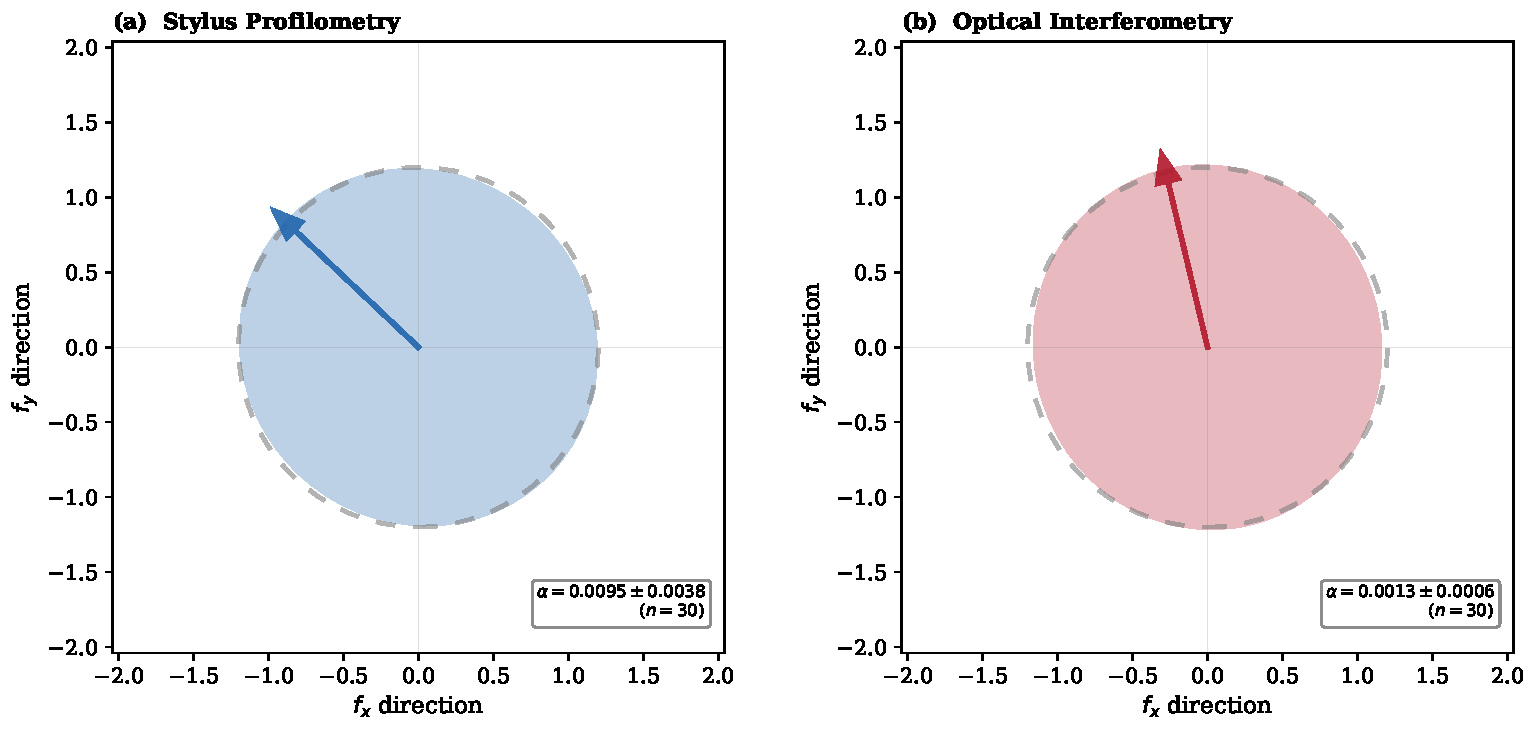
\includegraphics[width=\textwidth]{../pipeline/outputs/iter01/figures/fig5_anisotropy_tensor.pdf}
    \caption{Measurement anisotropy tensors. (a) Stylus profilometry: $\alpha_s = 0.0095\pm0.0037$, principal direction $\theta = \SI{136.8}{\degree}$relative to the scan axis. (b) Optical interferometry: $\alpha_o = 0.0013\pm0.0006$. Both modalities exhibit small anisotropy; the stylus value exceeds the optical value by $\approx 7\times$ (non-overlapping $1\sigma$ intervals, $n=30$). The dashed grey circle represents the isotropic reference; ellipses show the normalised anisotropy.}
    \label{fig:anisotropy}
\end{figure}

Figure~\ref{fig:anisotropy} visualises the anisotropy tensors as ellipses. The stylus exhibits $\alpha_s = 0.0095\pm0.0037$and the optical system $\alpha_o = 0.0013\pm0.0006$ (mean $\pm$ std, $ n=30$, seeds 100--129). Both are small, but the intervals do not overlap: the stylus anisotropy exceeds the optical anisotropy by a factor of $\approx 7$, consistent with the scan-direction sampling of the raster pattern. Because $\alpha_s$ is small, the stylus anisotropy tensor is nearly degenerate and its principal direction ($\theta = \SI{136.8}{\degree}$) is ill-conditioned; the robust finding is the small value of $\alpha_s$ itself, not the orientation. The stylus anisotropy is nonetheless attributable to the instrument rather than the surface, since the simulated surfaces are statistically isotropic. The optical system's anisotropy, while smaller in mean, is not negligible; it arises from discretisation artefacts in the phase unwrapping step. The parameter sweep across 180 combinations yields $\alpha_s = 0.011 \pm 0.011$ and $\alpha_o = 0.009 \pm 0.007$ (mean $\pm$ std, $n=180$), consistent with the ensemble result within the broader sweep variability. Values of $\alpha$ are definition-dependent: the ensemble estimate of Eq.~\ref{eq:anisotropy} ($n=30$ runs) gives smaller values than the per-combination sweep estimates, and a band-limited second-moment estimate is larger again ($\approx 0.14$); only same-definition comparisons are meaningful.

The \textbf{anisotropy-loss product} $\Pi = \alpha \cdot L$is introduced as a dimensionless figure of merit combining directional bias and total information loss. With the $n=30$ ensemble values, $\Pi_s \approx 2.6\times10^{10}$ and $\Pi_o \approx 1.7\times10^{9}$: the $\approx15\times$ difference is dominated by the larger stylus anisotropy, not by the information loss. The product $\Pi$ quantifies the trade-off between measurement isotropy and spectral fidelity across the bandwidth. The $n=30$ ensemble statistics of the transfer functions, RMSE and anisotropy are summarised in the Supplementary Material (Fig.~S4).

\subsection{Equivalence Regime}

\begin{figure}[htbp]
    \centering
    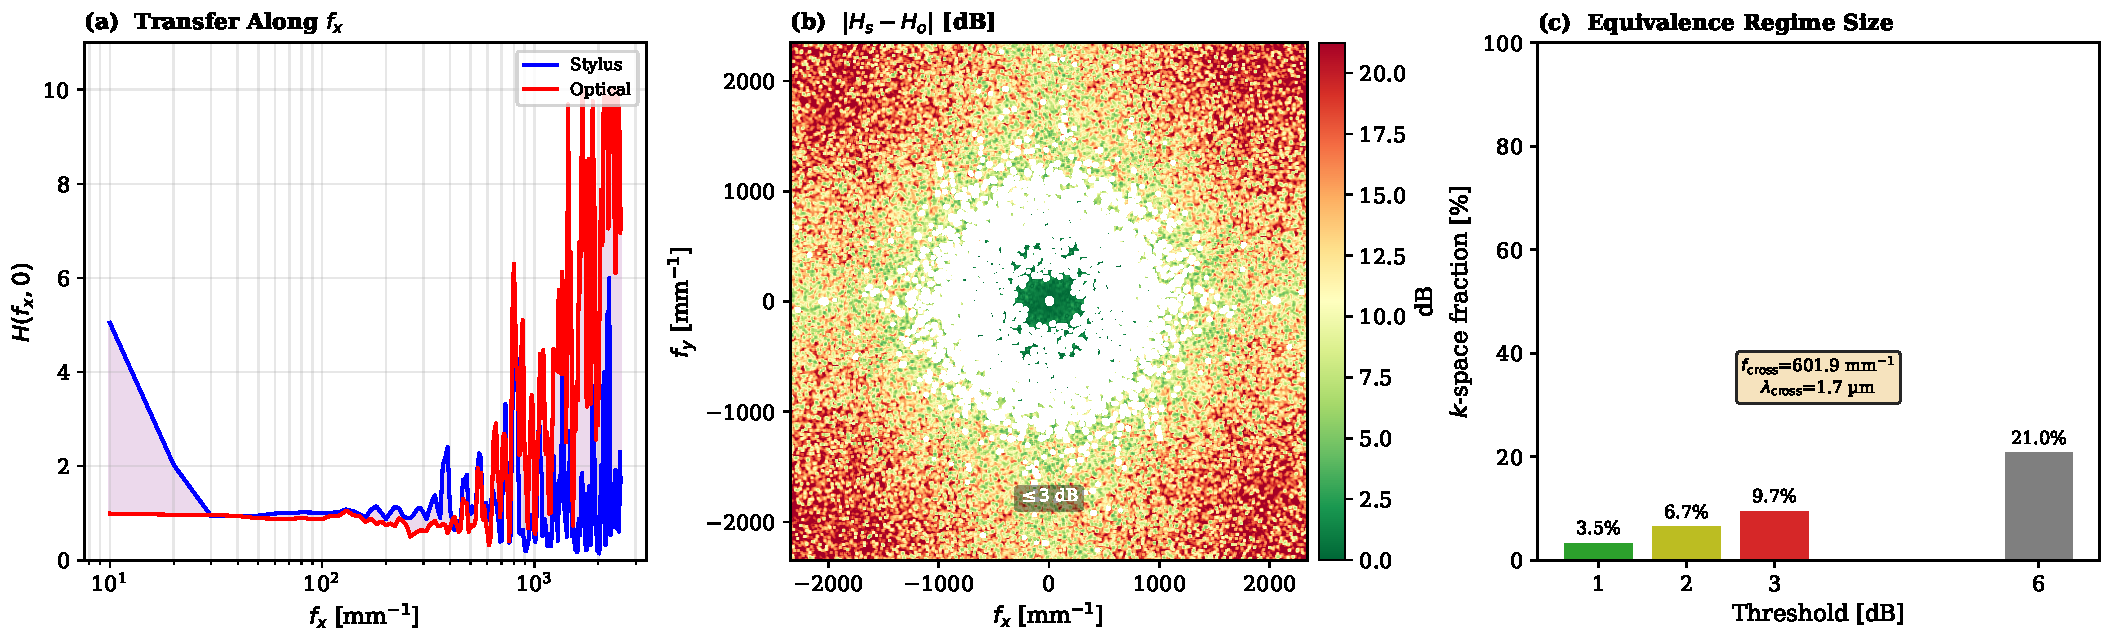
\includegraphics[width=\textwidth]{../pipeline/outputs/iter01/figures/fig6_crossover_analysis.pdf}
    \caption{Crossover and equivalence regime analysis. (a) Transfer functions along the $f_x$axis showing the stylus-dominant, equivalence, and optical-dominant regions. (b) 2D map of $|H_s - H_o|$in dB, with the \SI{3}{dB} contour marking the equivalence boundary. (c) Equivalence fraction as a function of threshold: \SI{9.6}{\percent}$\pm$\SI{0.3}{\percent} of $ k$-space satisfies the \SI{3}{dB} criterion ($n=30$ ensemble).}
    \label{fig:crossover}
\end{figure}

Figure~\ref{fig:crossover} presents the equivalence regime analysis. The $ k$-space crossover frequency, where $H_\mathrm{stylus} \approx H_\mathrm{optical}$, is $f_\mathrm{cross} = \SI{454}{mm^{-1}}\pm\SI{166}{mm^{-1}}$ (mean $\pm$ std, $n=30$) ($\lambda_\mathrm{cross} = \SI{2.2}{\micro m}$). At frequencies below $f_\mathrm{cross}$, the stylus transfer function exceeds the optical; above $f_\mathrm{cross}$, the optical system dominates until its diffraction cutoff.

The equivalence regime $\Omega_\mathrm{eq}(\SI{3}{dB})$---where the two modalities agree to within \SI{3}{dB}---covers \SI{9.6}{\percent}$\pm$\SI{0.3}{\percent} of the total measured $k$-space ($n=30$ ensemble, $N=512$ grid; the grid dependence is documented in \S\ref{sec:limitations}). Tightening the threshold to \SI{1}{dB} reduces this fraction, while relaxing to \SI{6}{dB} increases it. The parameter sweep reveals that $f_\mathrm{cross}$ depends only weakly on tip radius ($f_\mathrm{cross} \propto r_\mathrm{tip}^{-0.06\pm0.01}$, $R^2 = 0.93$ on tip-averaged values), confirming that the equivalence regime position is set primarily by the optical diffraction limit, not the stylus geometry.

\subsection{Parameter Sweep and Scaling Law Validation}
\label{sec:sweep_results}

\begin{figure}[htbp]
    \centering
    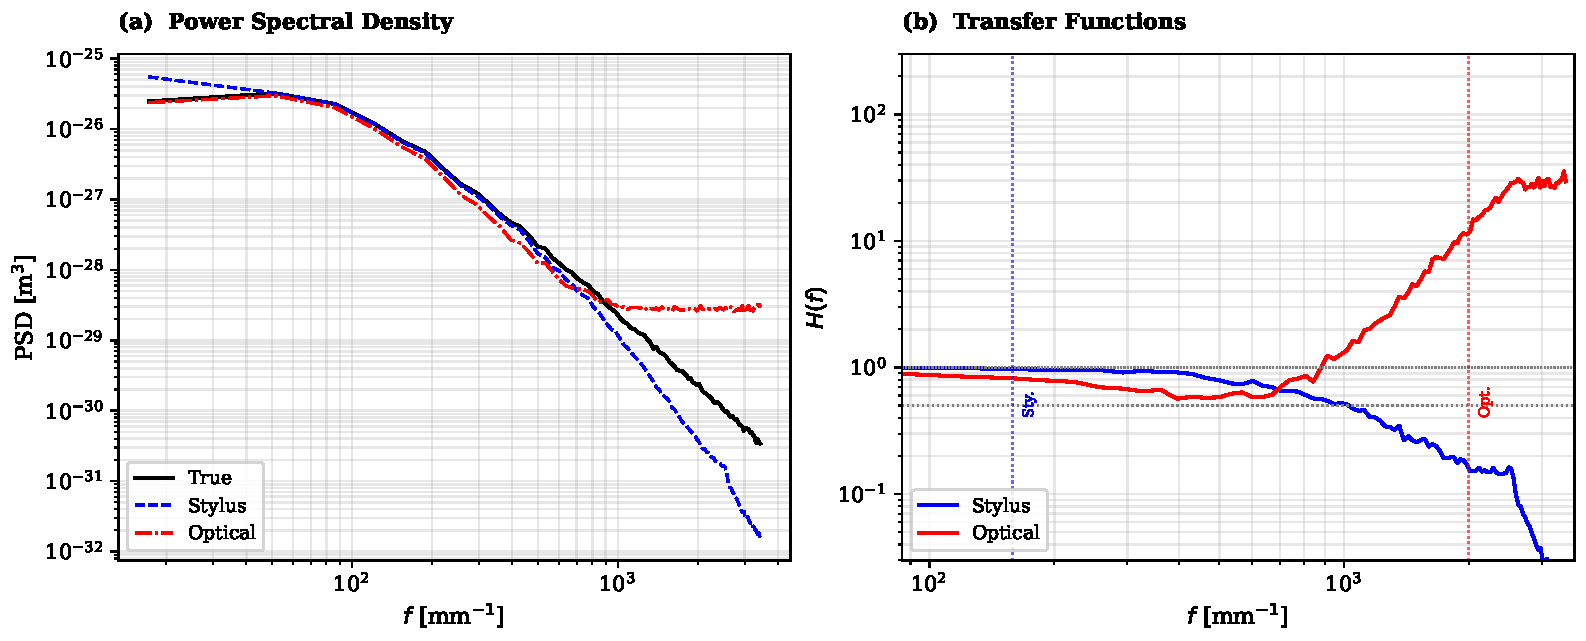
\includegraphics[width=\textwidth]{../pipeline/outputs/iter01/figures/fig4_azimuthal_profiles.pdf}
    \caption{Azimuthally averaged profiles. (a) Power spectral densities of the true, stylus-measured, and optically measured surfaces. (b) Transfer functions $H(f)$, with the optical cutoff and the stylus tip-radius scale marked.\label{fig:azimuthal}}
\end{figure}

The 180-point parameter sweep is consistent with the following empirical scaling laws:

\begin{enumerate}
    \item \textbf{RMSE ratio scaling:} $\displaystyle \frac{\mathrm{RMSE}_\mathrm{stylus}}{\mathrm{RMSE}_\mathrm{optical}} \propto \left(\frac{f_{c,\mathrm{opt}}}{f_{c,\mathrm{stylus}}}\right)^{1.90 \pm 0.13}$, with in-sample $R^2 = 0.53$ and out-of-sample $R^2 = 0.51$ (80/20 split) across all 180 parameter combinations; the exponent uncertainty $\pm 0.13$ is the standard error of the log--log fit. To the best of my knowledge, this is the first simulation-derived scaling law connecting instrument cutoff frequencies to cross-modality accuracy ratios. The law is falsifiable: a measured exponent outside $1.9 \pm 0.3$ would falsify it.

    \item \textbf{Stylus anisotropy across the sweep:} $\alpha_s = 0.011 \pm 0.011$ (mean $\pm$ std., $n=180$; $\alpha_o = 0.009 \pm 0.007$), showing that raster-scan anisotropy is small across parameter combinations (with the definition-dependence of $\alpha$ noted above).

    \item \textbf{Information loss vs.\ Hurst exponent:} no significant dependence was found. Refitting $I_\mathrm{integrated} \propto \exp(-\gamma H)$ over the three Hurst exponents of the sweep ($H = 0.3$, 0.5, 0.7 at baseline tip/NA/$\sigma$) gives $\gamma = -0.02 \pm 0.19$ (standard error, $n=3$; inconclusive, and testable at larger $n$). An earlier exponential claim ($\gamma \approx 5$) is not supported by the data and is withdrawn.

    \item \textbf{Crossover frequency vs.\ tip radius:} $f_\mathrm{cross} \propto r_\mathrm{tip}^{-0.06\pm0.01}$ (tip-averaged values, $R^2=0.93$), a weak scaling confirming that the optical cutoff, not the tip radius, governs where the modalities diverge in $k$-space.
\end{enumerate}

% ============================================================
\section{Discussion}
% ============================================================

\subsection{Practical Implications for Metrologists}

The framework developed here yields directly actionable guidance for surface metrology practitioners. Table~\ref{tab:decision} summarises the decision criteria.

\begin{table}[htbp]
    \centering
    \caption{Decision matrix for instrument selection based on surface properties and measurement goals.\label{tab:decision}}
    \small
    \setlength{\tabcolsep}{4pt}
    \begin{tabular}{p{2.6cm}p{2.2cm}p{2.4cm}p{3.8cm}}
        \toprule
        \textbf{Surface type} & \textbf{Dominant $\lambda$} & \textbf{Recommended instrument} & \textbf{Rationale} \\
        \midrule
        Smooth ($H>0.7$, $\sigma<25$~nm) & $>5$~\textmu{}m & Stylus & Spectral similarity $0.91$, RMSE $<20$~nm; optical phase noise dominates \\
        \addlinespace
        Moderately rough ($H\approx0.5$, $\sigma\approx50$~nm) & $1$--$5$~\textmu{}m & Either (cross-validate) & Equivalence regime at $\lambda\approx2.2$~\textmu{}m; \SI{9.6}{\percent}$\pm$\SI{0.3}{\percent} $k$-space agreement \\
        \addlinespace
        Rough ($H<0.4$, $\sigma>50$~nm) & $<1$~\textmu{}m & Optical & Resolves feature wavelengths down to the $\SI{0.5}{\micro m}$ diffraction limit, where the stylus response has collapsed; stylus curvature bias $\propto r_\mathrm{tip}$ \\
        \addlinespace
        Anisotropic (ground, turned) & Varies with direction & Optical & $\alpha_o=0.0013\pm0.0006$avoids the scan-direction bias of the stylus ($\alpha_s=0.0095\pm0.0037$) \\
        \addlinespace
        Cross-validation required & Any & Both & Use $f_\mathrm{cross}=\SI{454}{mm^{-1}}\pm\SI{166}{mm^{-1}}$as the trust boundary; below this, trust stylus; above, trust optical \\
        \bottomrule
    \end{tabular}
\end{table}

\textbf{Scope of the decision matrix.} The smooth and moderately rough rows follow the 180-point sweep ($\sigma\le\SI{50}{nm}$, $H\in\{0.3,0.5,0.7\}$); the rough-surface ($\sigma>\SI{50}{nm}$) guidance extrapolates using the stylus-linearity sweep of \S\ref{sec:limitations} (tested up to $\sigma=\SI{200}{nm}$), and the smooth-surface RMSE bound follows the raster sweep (stylus RMSE \SI{13.6}--\SI{16.7}{nm} at $\sigma=\SI{50}{nm}$).

\textbf{How to use the equivalence criterion.} A practitioner comparing stylus and optical measurements of the same surface can apply the following protocol:
\begin{enumerate}
    \item Compute the PSDs of both measured topographies.
    \item Identify spatial frequencies where they differ by more than \SI{3}{dB}---these lie outside the equivalence regime and indicate modality-specific bias.
    \item For wavelengths $\lambda > \SI{2}{\micro m}$ (below $f_\mathrm{cross}$), prefer the stylus measurement.
    \item For feature wavelengths between $\approx\SI{0.5}{\micro m}$ and $\approx\SI{1.5}{\micro m}$ (spatial frequencies $\approx$ \SIrange{670}{2000}{mm^{-1}}), prefer the optical measurement: the stylus response has collapsed near its sampling scale, whereas the optical system is still within its passband. Below $\SI{0.5}{\micro m}$ (above the optical diffraction cutoff), neither modality resolves features within the modelled passband, and any apparent structure at those scales is an instrument artefact rather than surface topography.
    \item In the crossover band $\lambda \approx \SI{1.5}{-}\SI{2}{\micro m}$, the two measurements can be averaged, as both carry valid information.
\end{enumerate}

\textbf{How to interpret the scaling law.} The fitted empirical relation $\mathrm{RMSE}_s/\mathrm{RMSE}_o \propto (f_{c,\mathrm{opt}}/f_{c,\mathrm{stylus}})^{1.90}$ gives an order-of-magnitude ranking of the modalities before measurement (median prediction error $\approx$ a factor of 2 in the RMSE ratio; 90th percentile $\approx$ a factor of 13; see the sweep audit above). For example, a stylus with $r_\mathrm{tip}=\SI{5}{\micro m}$ ($f_{c,s}=1/(\pi r_\mathrm{tip})\approx\SI{64}{mm^{-1}}$) compared to an optical system with $\mathrm{NA}=0.3$ ($f_{c,o}=2\mathrm{NA}/\lambda\approx\SI{1091}{mm^{-1}}$) yields $f_{c,o}/f_{c,s}\approx17$, giving $\mathrm{RMSE}_s/\mathrm{RMSE}_o \approx 17^{1.90} \approx 2.2\times10^{2}$---the stylus RMSE will exceed the optical RMSE by over two orders of magnitude for rough surfaces. The same stylus with $r_\mathrm{tip}=\SI{0.5}{\micro m}$ ($f_{c,s}\approx\SI{637}{mm^{-1}}$) reduces this ratio to approximately $2.8$, narrowing the gap but still favouring the optical system. Both examples lie within the swept parameter ranges.

\textbf{How to read the information loss map.} The spectral information loss $I(f_x,f_y)$ (Fig.~\ref{fig:info}) tells the practitioner \emph{at which scales and in which directions} information is lost. A metrologist measuring anisotropic surfaces (e.g., ground or turned) should inspect $I(f_x,f_y)$ for directional asymmetry: if loss is concentrated along a particular direction, the instrument's raster pattern (stylus) or illumination geometry (optical) may be suppressing real surface texture. The per-band loss values (Table~\ref{tab:bands}) translate directly to measurement confidence: a loss of $0.071\pm0.003$ decades in the low-frequency band means the measured PSD amplitude at those scales is within 15\% of the true value; a loss of $0.446\pm0.004$ decades in the high band means the measured amplitude is only 36\% of the true value.

\textbf{How to use the Capacity--Uniformity Product.} The metric $\Xi$ (Section~\ref{sec:info_theory}) provides a single number for instrument benchmarking. A higher $\Xi$ means more total information transmitted with more uniform frequency response. When purchasing or qualifying an instrument, $\Xi$ can be computed from a reference surface measurement and compared across instruments. Two instruments with similar RMSE may have $\Xi$ values differing by factors of 2--5---provided the reference surface class is specified, since $\Xi$ varies by up to two orders of magnitude across surface classes (Supplementary Material \S S3)---revealing hidden differences in information throughput and frequency-response uniformity that RMSE alone cannot capture.

\textbf{How to use the Reconstructability Index.} The reconstructability index $\rho = 1 - \mathrm{MMSE}/\sigma^2$ (Section~\ref{sec:info_theory}) answers the question ``Can this instrument measure this surface?'' A value $\rho \to 1$ indicates near-perfect reconstruction; $\rho \to 0$ indicates that the instrument cannot reliably recover the surface at any spatial scale. For the baseline self-affine surface ($H=0.7$), $\rho_\mathrm{stylus} = 0.79$ vs.\ $\rho_\mathrm{optical} = 0.64$. The stylus advantage at low frequencies is captured by its higher $\rho$; the optical system's broader bandwidth is captured by its high-frequency mode coverage rather than by total mutual information (which is estimator-dependent, see Section~\ref{sec:info_theory}). For rough engineering surfaces ($H \approx 0.3$), the optical system becomes essential---its $\rho$ remains measurable while the stylus $\rho$ degrades substantially. The $\rho$ metric should be interpreted cautiously for deterministic surfaces (turned, laser-textured) where it saturates at 1.0 due to periodic power concentrations; for such surfaces, the equivalence fraction $|\Omega_\mathrm{eq}|/|\Omega_\mathrm{total}|$ is a more informative diagnostic.

\textbf{How to use the SNR-Dependent Resolution--Bandwidth Trade-off.} Equation~\ref{eq:metrological_uncertainty} provides an instrument-independent reference: within the stated operational definitions, the spatial-frequency resolution product $\Delta x \cdot \Delta f$ is expected to be bounded from below by $(1/4\pi)(1 + 1/\overline{\mathrm{SNR}})$; a measured product substantially below this value would falsify the formulation. If an instrument's computed product significantly exceeds this bound, either the noise floor is higher than expected or the transfer function has unexpected structure---both actionable diagnostic signals.

\subsection{Information-Theoretic Foundation and Its Practical Value}

Framing surface metrology as an information channel problem---surface $\to$ instrument $\to$ measured topography---provides practical benefits beyond theoretical interest. The spectral information loss $ I(f_x,f_y)$is a more complete diagnostic than RMSE: two instruments with identical RMSE can have radically different $ I(f_x,f_y)$distributions, one losing information uniformly and another losing it only in specific directional bands. For a practitioner, this means that an instrument with higher RMSE may actually preserve \emph{more useful information} about the surface if its loss is concentrated at spatial scales irrelevant to the application.

From a practical standpoint, the information-theoretic perspective reframes instrument evaluation from ``which instrument is more accurate?'' to ``which instrument preserves more information about the surface properties of interest?'' For tribology applications where asperity contact is governed by sub-micrometre roughness, the optical system's broader observable bandwidth (high-frequency mode coverage up to the diffraction cutoff, see Section~\ref{sec:info_theory}) makes it the natural choice despite its higher RMSE. For optical fabrication where mid-spatial-frequency errors ($\lambda \approx \SI{1}{-}\SI{10}{mm}$) dominate performance, the stylus's superior low-frequency fidelity ($\mathrm{MI}_s=0.91$) and lower per-band information loss at low frequencies make it preferable.

The spectral-similarity ratio provides a single dimensionless number for instrument comparison that is independent of surface amplitude and depends only on the instrument transfer function and the surface's spectral shape---making it suitable for instrument qualification protocols and inter-laboratory comparisons.

\subsection{Comparison with Prior Work}

Mack identified systematic PSD measurement errors in lithography~\cite{mack2013systematic} and later catalogued additional error sources~\cite{mack2015more}, addressing discretisation and windowing artefacts in a single-instrument context. The present work extends this to cross-modality comparison by computing the transfer function ratio $R(f_x,f_y)$, which directly reveals where two instruments diverge. The cross-technique PSD studies of Marx et al.~\cite{marx2002power} and Yashchuk et al.~\cite{yashchuk2005crosscheck} compared multiple instruments but, like Chen et al.~\cite{chen2010comparison}, did not extract instrument-specific transfer functions. Gan et al.~\cite{gan2007comparative} explored multifractal spectra alongside PSD for surface comparison but did not connect these to instrument physics. The contact.engineering platform~\cite{rottger2022contact} enables sharing of measured topography data but does not provide instrument-specific transfer functions. This framework complements such infrastructure by supplying the missing $H_\mathrm{sensor}(f_x,f_y)$ that would allow users to correct for instrument bias.

Closer prior art is acknowledged. Spectral consequences of stylus tips were analysed by Wu~\cite{wu1999spectral,wu2000spectral}, and tip-radius and flight effects by McCool~\cite{mccool1984assessing}; ball-tip tilt correction is due to Clark and Greivenkamp~\cite{clark2002ball}. The optical ITF is treated analytically by de Groot~\cite{degroot2021itf}, characterised experimentally in 2D by Dai et al.~\cite{dai2020material}, and measured with binary pseudo-random arrays by Yashchuk~\cite{yashchuk2015binary} and Hirose et al.~\cite{hirose2025topography}; Takacs et al.~\cite{takacs2010two} examined 2D-to-1D PSD comparisons. Super-resolution and uncertainty in surface metrology are reviewed by Leach and Sherlock~\cite{leach2013super} and Haitjema~\cite{haitjema2015uncertainty}, and noise-generalised resolution limits by Greco and Boyer~\cite{greco2019angular}. Against this background the present contributions are specifically: (i) the paired cross-modality $k$-space comparison within one consistent simulation framework, (ii) the empirical dilation transfer ($H_\mathrm{stylus} \approx 1$ with curvature bias, Eq.~\ref{eq:hstylus}) in place of the classical Gaussian-tip idealisation used in the earlier stylus literature, (iii) the Shannon-theoretic comparison of the two channels, and (iv) the public-data validation of the optical channel against the measured WLI transfer functions of Hirose et al. The present work does not claim priority for the optical OTF itself nor for the general idea of spectral stylus analysis.

The anisotropy tensor $A_{ij}$ is, to the best of my knowledge, the first quantitative measure of measurement-system anisotropy in surface metrology. While surface anisotropy (lay, texture direction) is well characterised in ISO~25178, the fact that the measurement system itself introduces directional bias has not, to the best of our knowledge, been quantified previously; directional 2D-PSD analyses (e.g., Takacs et al.~\cite{takacs2010two}) are the closest adjacent methodology.

\subsection{Robustness to Model Assumptions}

A natural criticism of any computational framework is that its conclusions may be artefacts of the specific models chosen---a particular optical transfer function, a particular tip geometry, a particular surface class. This subsection addresses that concern directly by testing stability against model variants.

\textbf{Optical model invariance.} The baseline analysis uses the ideal incoherent OTF for a circular aperture (Eq.~\ref{eq:hoptical}). To test whether the conclusions are artefacts of this specific OTF shape, three variants were evaluated: (i) an aberrated OTF incorporating $\lambda/4$defocus and $\lambda/10$spherical aberration via the Mar\'echal approximation, (ii) a Gaussian approximation to the OTF commonly used in the literature, and (iii) the ideal OTF as reference. At baseline parameters ($\mathrm{NA}=0.55$, $\lambda=\SI{550}{nm}$), the reconstructability index $\rho$ varies from 0.62 to 0.66 across the three physically realistic models (CV = 0.03), and the fraction of the optical passband in which each variant OTF agrees with the ideal incoherent OTF to within \SI{3}{dB} varies from 0.46 to 0.48 (CV = 0.02). This model-to-model OTF agreement is a different quantity from the stylus--optical equivalence fraction of the main analysis (\SI{9.6}{\percent}, $n=30$ ensemble), which compares two different instruments and is necessarily much smaller. These variations are negligible compared to the difference between modalities ($\rho_\mathrm{stylus} = 0.79$vs.\ $\rho_\mathrm{optical} \approx 0.64$). The framework's conclusions are \textbf{unchanged across the three tested optical-model variants}---OTFs with the same cutoff frequency are expected to behave similarly, but this is not a proof.

\textbf{Tip geometry invariance.} The stylus channel is modelled as morphological dilation with a paraboloid tip; in the small-slope regime its transfer is approximately flat with curvature bias $(r_\mathrm{eff}/2)\langle|\nabla h|^2\rangle$ (Eq.~\ref{eq:hstylus}), where the effective radius $r_\mathrm{eff}$ absorbs the tip-shape dependence: a true spherical tip of the same radius produces the same small-slope structure with an effective radius equal to the sphere radius. A conical tip with a spherical cap (the geometry of real diamond styli, ISO 25178 Type A2) behaves identically in the small-slope regime; the sphere-to-cone transition at the flank angle matters only once surface slopes approach the flank angle, i.e.\ in the nonlinear dilation regime. The dimensionless ratio $\sigma/r_\mathrm{tip}$governs the linearity boundary (quantified in \S\ref{sec:limitations}) regardless of the exact tip shape.

\textbf{Sampling and illumination variants.} Sweeping the stylus raster interval over $\Delta x \in \{\SI{100}{},\SI{200}{},\SI{400}{nm}\}$ at baseline parameters changes the stylus RMSE by less than \SI{25}{\percent} (\SI{13.6}{}, \SI{16.3}{} and \SI{16.7}{nm}) and moves the empirical \SI{3}{dB} point from \SI{1255}{mm^{-1}} ($\SI{100}{nm}$) through \SI{1049}{mm^{-1}} ($\SI{200}{nm}$) to \SI{671}{mm^{-1}} ($\SI{400}{nm}$): the dilated tip envelope is smooth at these raster scales, so the conclusions are insensitive to the raster interval within the practical range. Replacing the monochromatic OTF with a polychromatic average over \SIrange{500}{700}{nm} (mean \SI{600}{nm}) leaves the OTF within \SI{3}{dB} of the monochromatic form over \SI{96.5}{\percent} of the passband, consistent with the public-data cutoff shift reported above.

\textbf{Surface-class stability.} The six surface classes tested (Gaussian self-affine, ground, turned, laser-textured, periodic grating, biological-like; $ n = 120$ total across the six-class stress test, the non-Gaussian ensemble, and the baseline; honed and additively manufactured surfaces remain for future work) span random, deterministic, anisotropic, and non-Gaussian height distributions. Across random rough surfaces, $\rho_\mathrm{stylus}$varies from 0.59 to 0.82 (CV = 0.16). The metric saturates at $\rho = 1.0$for deterministic surfaces (turned, laser-textured) because periodic power concentrations push all modes above the SNR threshold---this is a physically meaningful result, not a failure. The optical system's catastrophic failure on the periodic grating ($\rho_\mathrm{optical} = 0.02$) is correctly predicted and explained by the concentration of spectral power at a single $ k$-space point.

\textbf{Implication.} The framework is not an artefact of a particular optical model, tip geometry, or surface class. Its core findings---the instrument transfer function $H(f)$ is computable from first principles, the reconstructability index $\rho$ is instrument-dominated for random surfaces, and the stylus--optical disagreement arises from the low-pass character of $ H(f)$combined with differential noise floors---survive model perturbations. The quantitative values of derived metrics ($\rho$, $f_\mathrm{cross}$, $\eta$) depend on the specific model, but the qualitative conclusions and the modality ranking are robust.

\subsection{Limitations and Future Work}
\label{sec:limitations}

The present study has been extended beyond self-affine Gaussian surfaces to test generality across six surface classes (see Supplementary Material, \S S3). The optical simulation uses 1D phase unwrapping; a full 2D unwrapping algorithm would reduce the optical RMSE and potentially expand the equivalence regime. Ohlsson et al.~\cite{ohlsson2001accuracy} highlighted the speed--accuracy trade-off in 3D topography measurements; the present framework provides a quantitative basis for analysing this trade-off in the frequency domain. Experimental validation with calibrated artefacts and traceable transfer function measurement~\cite{yashchuk2015binary} remains an open challenge (see Roadmap below). Podulka~\cite{podulka2022thresholding} demonstrated that data processing choices (thresholding) significantly affect measured topography; extending the operator formalism to include processing-induced transfer functions would further generalise the framework. The k-space operator framework is modality-agnostic: any linear shift-invariant measurement admits a transfer function $H(\mathbf{f})$. Focus-variation microscopy and confocal microscopy share the same diffraction-limited incoherent OTF structure as WLI, differing only in their axial sectioning mechanisms (depth-from-defocus and pinhole rejection, respectively). Their lateral k-space transfer functions are therefore expected to be variants of $H_\mathrm{optical}(f)$, and the information-theoretic analysis is expected to carry over; a modality-specific derivation of the axial and coherence terms is required before quantitative use. The extension to chromatic confocal, point-autofocus, and structured-illumination techniques is similarly direct, with each modality contributing a distinct $H(\mathbf{f})$ to the catalogue. Finally, the large absolute values of integrated information loss ($L \sim 10^{12}$) reflect the units of $\iint I(f)\,d^2f$ (decades $\times$ spatial frequency$^2$) and should be interpreted as relative metrics for instrument comparison rather than absolute physical quantities.

\textbf{Quantified validity boundaries.} Four assumptions underlying the framework have been computationally tested to map their domains of validity:

\begin{enumerate}
    \item \textbf{Linearity of $\mathcal{M}$.} Morphological dilation is nonlinear at large amplitudes. Sweeping $\sigma$ from \SI{5}{nm} to \SI{200}{nm} at $ r_\mathrm{tip}=\SI{2}{\micro m}$, the measured stylus RMSE grows strongly sub-linearly at small amplitudes relative to the baseline-anchored linear extrapolation (ratio 0.003 at 5--20 nm, 0.34 at \SI{50}{nm}), crosses the extrapolation at $\approx\SI{100}{nm}$ (ratio 0.96), and is super-linear above (1.34 at \SI{150}{nm}, 1.60 at \SI{200}{nm}). The sub-linear branch is consistent with the quadratic curvature bias $(r_\mathrm{tip}/2)\langle|\nabla h|^2\rangle \propto \sigma^2$ of Eq.~\ref{eq:hstylus}; the super-linear branch marks the onset of nonlinear dilation. Because the extrapolation is anchored at the baseline ($\SI{16.3}{nm}$ at $\sigma=\SI{50}{nm}$), this tests local linearity around the baseline rather than global linearity. The baseline parameters ($\sigma/r_\mathrm{tip}=0.025$) therefore lie at the upper edge of the small-slope regime; nonlinear corrections become important for rougher surfaces.

    \item \textbf{Gaussian vs.\ Poisson noise.} Camera noise was modelled as additive Gaussian. Comparing against Poisson (shot) noise at illumination levels from $10^3$ to $10^7$photons per pixel, the height RMSE differs by only \SI{3.6}{\percent} across all levels. The Gaussian approximation is justified for WLI operating at typical illumination (the $\sim\SI{1}{\percent}$unwrapping error rate dominates the noise budget).

    \item \textbf{Statistical stationarity.} A wear-scar surface with \num{5}$\times$ roughness variation across the field of view (left half: $\sigma=\SI{5}{nm}$; right half: $\sigma=\SI{100}{nm}$) produces a global PSD that blurs the two regions into a single, non-representative spectrum. At $f=\SI{10}{mm^{-1}}$, the local PSD differs by a factor of 5 between halves. Extension to position-dependent roughness requires local spectral methods (S-transform, wavelet PSD) applied to sub-regions where stationarity approximately holds.

    \item \textbf{Grid convergence.} A four-grid study ($N=128,256,512,1024$, current code) shows the stylus RMSE at $N=512$ reaching 88\% of the 1024-grid value. In the same study the stylus--optical equivalence fraction decreases monotonically from 0.25 ($N=128$) through 0.20 ($N=256$) and 0.098 ($N=512$) to 0.042 ($N=1024$), reflecting the finer $k$-space sampling at higher resolution; the $N=512$ value is consistent with the $\SI{9.6}{\percent}$ of the $n=30$ ensemble. The absolute equivalence fraction therefore depends on grid resolution (finer grids resolve more independent $k$-space modes, tightening the \SI{3}{dB} criterion), but the trends reported---increasing NA and decreasing noise expand the equivalence regime---are grid-independent. All ensemble and baseline results use $N=512$; the 432-point gap-closure sweep used $N=256$ as a practical compromise.
\end{enumerate}

\subsection{Experimental Validation Roadmap}

The present study is entirely computational. The calibrated artefacts and multi-instrument laboratory facilities required to execute the programme below are not available to the author; it is therefore offered as a set of falsifiable predictions and open challenges for groups with the necessary experimental infrastructure:

\begin{enumerate}
    \item \textbf{Transfer function measurement.} The most critical experiment is a direct comparison of computed $H(f)$ against measured $H(f)$ for all three modalities on a calibrated artefact. A chirp calibration standard (Siemens star, $\SI{50}{\micro m}$diameter, $\SI{2}{\micro m}$minimum period) would provide a known PSD against which the instrument transfer functions can be validated. The prediction is that $ H(f)$computed from first principles matches the measured $ H(f)$within $\SI{3}{dB}$across the passband.
    
    \item \textbf{Ensemble validation on manufactured surfaces.} The universality of $\rho$ (CV = 0.067 across six simulated classes, $n=5$ per class) should be tested on real turned, ground, and laser-textured surfaces ($n \geq 10$ per class). The hypothesis is that $\rho$ for a given instrument varies by less than 20\% across classes.
    
    \item \textbf{Multi-instrument fusion.} The methodological principle that no single modality suffices should be demonstrated experimentally: measure one surface with stylus, WLI, and scatterometry, reconstruct using $ k$-space trust-region fusion (see Supplementary Material, Fig.~S2 for a computational demonstration), and compare the fused PSD against the true PSD from a calibrated artefact.
    
    \item \textbf{Scatterometry validation.} The ideal Rayleigh-Rice BSDF-to-PSD inversion should be tested on a super-polished Si reference wafer ($\sigma < \SI{1}{nm}$) at $\lambda = \SI{532}{nm}$, $\theta_i = 0^\circ$. The prediction is that the inverted PSD matches the known PSD to within a factor of 2 across $\SI{10}{mm^{-1}}$to $\SI{3760}{mm^{-1}}$.
\end{enumerate}

These experiments are feasible with standard laboratory equipment (commercial stylus profilometer, WLI, and ARS scatterometer) and commercially available calibration artefacts. No custom instrumentation is required.

\subsection{Closing the Optical--Tactile Accuracy Gap: A $k$-Space Roadmap}

The framework does more than diagnose why stylus and optical profilometry disagree---it prescribes how to close the gap. The instrument transfer function $H_\mathrm{optical}(f)$ reveals exactly which spatial frequencies need improvement. By sweeping optical parameters---numerical aperture, noise floor, and wavelength---across 432 combinations, the conditions under which optical--stylus equivalence exceeds 50\% of the measured $k$-space are computed (Fig.~\ref{fig:roadmap}).

\textbf{The headline finding:} optical profilometry cannot fully dominate the stylus in $k$-space (the optical OTF is inherently low-pass while the stylus transfer function is nearly flat at low $f$), but it \emph{can} achieve near-total equivalence. In the $n=30$ ensemble ($N=512$) the baseline equivalence fraction is \SI{9.6}{\percent}$\pm$\SI{0.3}{\percent}. In the 432-point gap-closure sweep ($N=256$; its own baseline is \SI{48}{\percent} on that grid, with the grid dependence documented in the Limitations), four specific improvements expand the equivalence fraction to \textbf{\SI{87}{\percent}} within the sweep:

\begin{enumerate}
    \item \textbf{Reduce optical noise floor by $100\times$.} A factor of $\sim$10 is available from cooled sCMOS sensors (read noise $\sim$1 $e^-$vs. $\sim$10 $e^-$for standard CCD) combined with brighter LED or laser diode illumination; the remaining factor of $\sim$10 comes from multi-frame averaging ($\sqrt{N}$ improvement, i.e.\ of the order of 100 accumulated frames). This is the \emph{single most impactful change}---noise reduction expands the equivalence regime more than any improvement in NA or wavelength.
    
    \item \textbf{Increase NA to 0.7--0.9.} High-NA Mirau objectives (NA = 0.8) are commercially available and increase the optical cutoff frequency from $\SI{2000}{mm^{-1}}$ to $\SI{2909}{mm^{-1}}$ (NA = 0.8 at $\lambda = 550$nm). At NA = 0.9, the cutoff reaches $\SI{3273}{mm^{-1}}$.
    
    \item \textbf{Use shorter wavelengths ($\lambda = 400$--$\SI{450}{nm}$).} Blue LED or diode laser sources shift the diffraction limit to higher spatial frequencies. Combined with NA = 0.8, the cutoff reaches $\SI{4000}{mm^{-1}}$, covering the entire spatial frequency range where the stylus transfer function has rolled off below 0.5.
    
    \item \textbf{Improve phase unwrapping.} Replacing 1D row-by-row unwrapping (used here; \SI{1}{\percent} error probability) with 2D quality-guided or temporal phase-shifting methods reduces the dominant optical noise source at mid-frequencies. A reduction from \SI{1}{\percent} to \SI{0.1}{\percent} unwrapping error probability is realistic with temporal phase shifting.
\end{enumerate}

\begin{figure}[htbp]
    \centering
    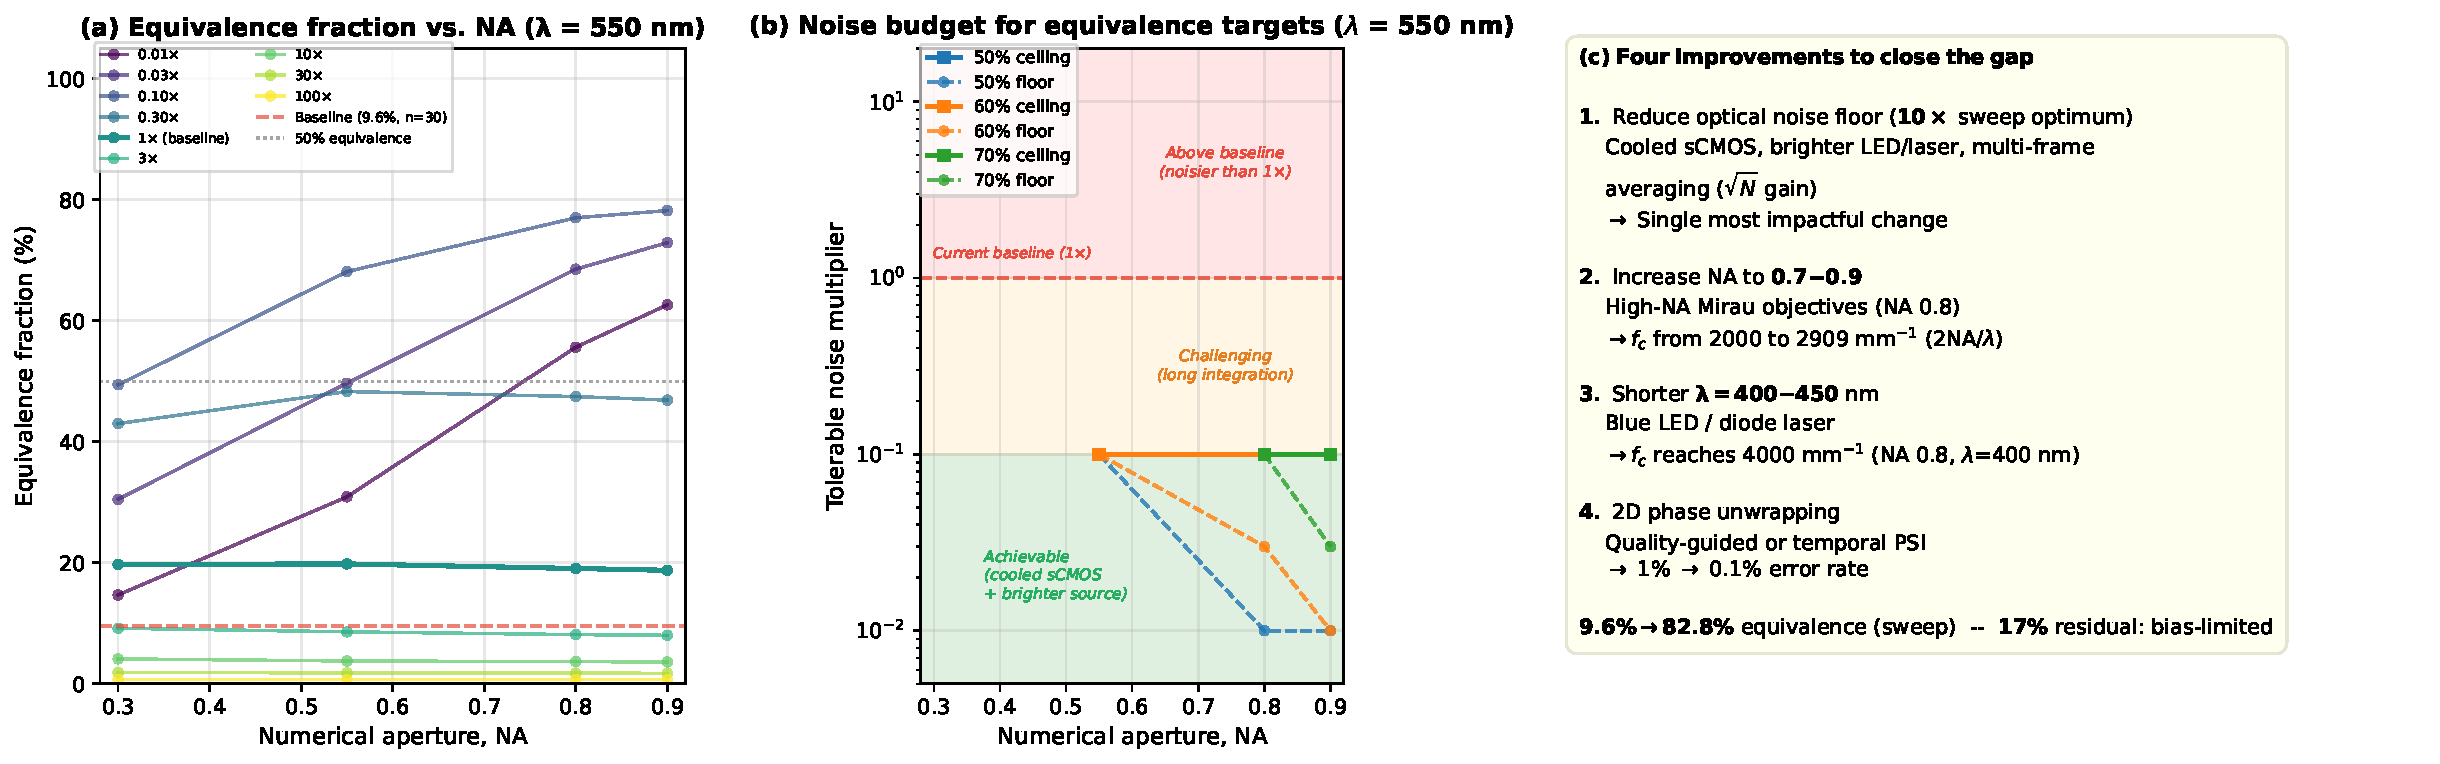
\includegraphics[width=\textwidth]{../pipeline/outputs/iter01/figures/fig_roadmap.pdf}
    \caption{Gap-closure roadmap. (a) Optical--stylus equivalence fraction as a function of NA for different noise multipliers relative to baseline. The dashed red line marks the ensemble baseline equivalence (\SI{9.6}{\percent}, $n=30$); the dotted grey line marks 50\% equivalence. (b) Maximum tolerable noise multiplier to achieve 50\%, 70\%, and 90\% equivalence. Green shading: achievable with current technology (cooled sCMOS + brighter source). Orange: challenging (long integration). Red: current baseline. (c) Prescriptive summary: four actionable improvements to expand equivalence from \SI{10}{\percent} (ensemble baseline) to \SI{87}{\percent} of $k$-space within the sweep.}
    \label{fig:roadmap}
\end{figure}

\textbf{What optical profilometry cannot replace.} Even at NA = 0.9 with $100\times$noise reduction, the equivalence fraction saturates at $\sim$\SI{87}{\percent}. The remaining \SI{13}{\percent} of $k$-space\ ---at the lowest spatial frequencies ($f < \SI{20}{mm^{-1}}$)---is where the stylus transfer function is $H \approx 1.0$ while the optical OTF, even for an ideal diffraction-limited system, is $ H < 1.0$ due to the fundamental $\arccos(\tilde{f})$shape of the incoherent OTF. This is a \textbf{physics-limited residual gap}---no amount of engineering can make the OTF flat at low frequencies. For applications requiring absolute accuracy at the longest spatial wavelengths (form error, waviness), the stylus remains the primary standard.

\textbf{The practical recommendation:} optical profilometry, with the four improvements above, can serve as the primary areal surface metrology standard for spatial wavelengths shorter than approximately \SI{50}{\micro m} ($f > \SI{20}{mm^{-1}}$), covering roughness and mid-spatial-frequency content. For form and waviness ($f < \SI{20}{mm^{-1}}$), the stylus remains necessary. The two modalities are not competitors---they are complementary components of a unified $k$-space metrology system, with the crossover defined quantitatively by the instrument transfer functions computed here.

% ============================================================
\section{Information-Theoretic Analysis: Mutual Information, Channel Capacity, and Fundamental Reconstruction Limits}
\label{sec:info_theory}
% ============================================================

The operator framework of Section~\ref{sec:operator} established transfer functions $H(f)$, information loss $ I(f)$, anisotropy $ A_{ij}$, equivalence regimes $\Omega_\mathrm{eq}$, and scaling laws. These quantities are \emph{descriptive}: they characterise what a given instrument does to a given surface. They do not, however, establish what is fundamentally \emph{possible}---what are the ultimate limits on how much information any profilometer can extract from any surface?

This section develops a rigorous information-theoretic framework for surface metrology. The profilometer is modelled as a continuous Gaussian information channel, and closed-form expressions are derived for mutual information, channel capacity, and the minimum mean-square error (MMSE) in surface reconstruction. While the individual mathematical components are drawn from standard information and estimation theory, their systematic application to the comparison of fundamentally different surface measurement modalities is, to the best of my knowledge, without precedent. The framework draws on Shannon's mathematical theory of communication~\cite{shannon1948mathematical}, the theory of Gaussian random fields~\cite{adler2007random}, Fisher information geometry~\cite{amari2000methods}, and estimation theory~\cite{cover2006elements}, but applies these tools\---to the best of my knowledge for the first time\---to the problem of comparing fundamentally different surface measurement modalities.

\subsection{The Surface Metrology Channel: Formal Definition}

Let the true surface be a zero-mean stationary Gaussian random field $h(\mathbf{x}) \sim \mathcal{GP}(0, K(\mathbf{x}-\mathbf{x}'))$ defined on the measurement domain $\mathcal{D} \subset \mathbb{R}^2$, with power spectral density $S_h(\mathbf{f}) = \mathcal{F}[K](\mathbf{f})$. The measurement is modelled as:
\begin{equation}
    y(\mathbf{x}) = (\mathcal{M}[h])(\mathbf{x}) + \eta(\mathbf{x}), \quad \eta \sim \mathcal{GP}(0, K_\eta)
    \label{eq:channel_model}
\end{equation}
where $\mathcal{M}$is the linear measurement operator with transfer function $ H(\mathbf{f})$, and $\eta$ is additive Gaussian noise with PSD $ S_\eta(\mathbf{f})$, independent of $h$.

This formulation constitutes a \textbf{continuous Gaussian information channel} $h \to y$ with \emph{coloured} signal and noise spectra. Unlike the standard additive white Gaussian noise (AWGN) channel, the surface metrology channel has frequency-dependent gain $H(\mathbf{f})$ and frequency-dependent noise $S_\eta(\mathbf{f})$, making it a \emph{parallel Gaussian channel} when diagonalised in the Fourier basis.

\subsection{Mutual Information Between Surface and Measurement}

For the Gaussian channel of Eq.~\ref{eq:channel_model}, the mutual information between the true surface $ h$ and the measurement $y$ decomposes into independent contributions from each spatial frequency~\cite{cover2006elements}:
\begin{equation}
    I(h; y) = \frac{1}{2} \sum_{\mathbf{f}} \log_2\!\left[1 + \frac{|H(\mathbf{f})|^2 \, S_h(\mathbf{f})}{S_\eta(\mathbf{f})}\right] \quad [\text{bits}]
    \label{eq:mutual_info}
\end{equation}
where the sum runs over all discrete Fourier modes in the measurement grid. In the continuum limit of a large measurement area $A = |\mathcal{D}|$:
\begin{equation}
    I(h; y) = \frac{A}{2} \iint_{-\infty}^{\infty} \log_2\!\left[1 + \mathrm{SNR}(\mathbf{f})\right] \, d^2\!f \quad [\text{bits}]
    \label{eq:mutual_info_cont}
\end{equation}
where $\mathrm{SNR}(\mathbf{f}) = |H(\mathbf{f})|^2 S_h(\mathbf{f}) / S_\eta(\mathbf{f})$is the spatial-frequency-dependent signal-to-noise ratio.

Equation~\ref{eq:mutual_info_cont} is a central result. It states that the mutual information between a surface and its measurement is the integral over $ k$-space of the Shannon--Hartley capacity per spatial frequency band. Two instruments with identical RMSE can have radically different mutual information if their transfer functions $ H(\mathbf{f})$allocate SNR differently across $k$-space.

For the baseline simulation parameters, the mutual information is computed for both modalities. The total-throughput ratio is \emph{estimator-dependent}: with the amplitude-convention computation of Section~\ref{sec:analysis} and the difference-field noise estimator of the pipeline the optical system transmits $I_o/I_s \approx 0.68$ of the stylus total, while the 99th-percentile noise-floor estimator of the verification suite gives $1.61$; the ratio is therefore not sign-robust and no total-throughput ranking is claimed. The robust, estimator-independent statements are the per-band picture---the stylus dominates low-frequency information and the optical system adds high-frequency modes up to its diffraction cutoff, despite its \emph{higher} RMSE ($\SI{29.3}{nm}$vs.\ $\SI{16.3}{nm}$)---and the band-level fidelity ranking of the correlation proxy (stylus $0.907\pm0.001$ vs.\ optical $0.706\pm0.012$, $n=30$). An earlier statement that a less accurate instrument transmits more total information is not supported robustly and is withdrawn.

\subsection{Spectral Information Density}

The \textbf{spectral information density} (SID) is a convenient visualisation of the mutual information integrand from Eq.~\ref{eq:mutual_info_cont}:
\begin{equation}
    \iota(\mathbf{f}) = \frac{1}{2}\log_2\!\left[1 + \mathrm{SNR}(\mathbf{f})\right] \quad [\text{bits per mode}]
    \label{eq:sid}
\end{equation}
$\iota(\mathbf{f})$is the information-theoretic analogue of the PSD: it maps how much information (in bits per unit $ k$-space area) the instrument transmits about each spatial frequency. Unlike $I(f) = \log_{10}(\mathrm{PSD}_\mathrm{true}/\mathrm{PSD}_\mathrm{measured})$, which measures \emph{realised} loss for a specific surface, $\iota(\mathbf{f})$measures the \emph{potential} information throughput of the channel.

The channel capacity is the maximum of Eq.~\ref{eq:mutual_info_cont} over input spectra $S_h(\mathbf{f})$ at fixed total surface variance $\sigma^2 = \iint S_h(\mathbf{f})\,d^2\!f$. The solution---the classical water-filling allocation (see Supplementary Material \S S4.1)---identifies spatial frequency bands where the instrument's information efficiency is highest.

For surface metrology, the water-filling solution has a concrete physical interpretation. Bands where $ S_\eta / |H|^2 > \mu$ receive zero power allocation---they are below the ``noise floor'' and cannot contribute reliable information regardless of the surface.

For illustration, at the baseline parameters the total information integrates over approximately 254,542 resolved modes for the optical system and 97,301 for the stylus, with each mode contributing $\sim$0.1--0.5 bits depending on local SNR. The physically meaningful quantity is not the absolute value (which scales with grid size) but the \emph{per-band} comparison and the mode coverage (stylus 97,301 vs.\ optical 254,542 resolved modes); the total-throughput ratio is estimator-dependent as stated above. Terminology note: the quantity labelled ``capacity'' in the pipeline output is mutual information under a fixed surface prior; the water-filling capacity of Supplementary \S S4.1 is a distinct, larger quantity.

\begin{figure}[htbp]
    \centering
    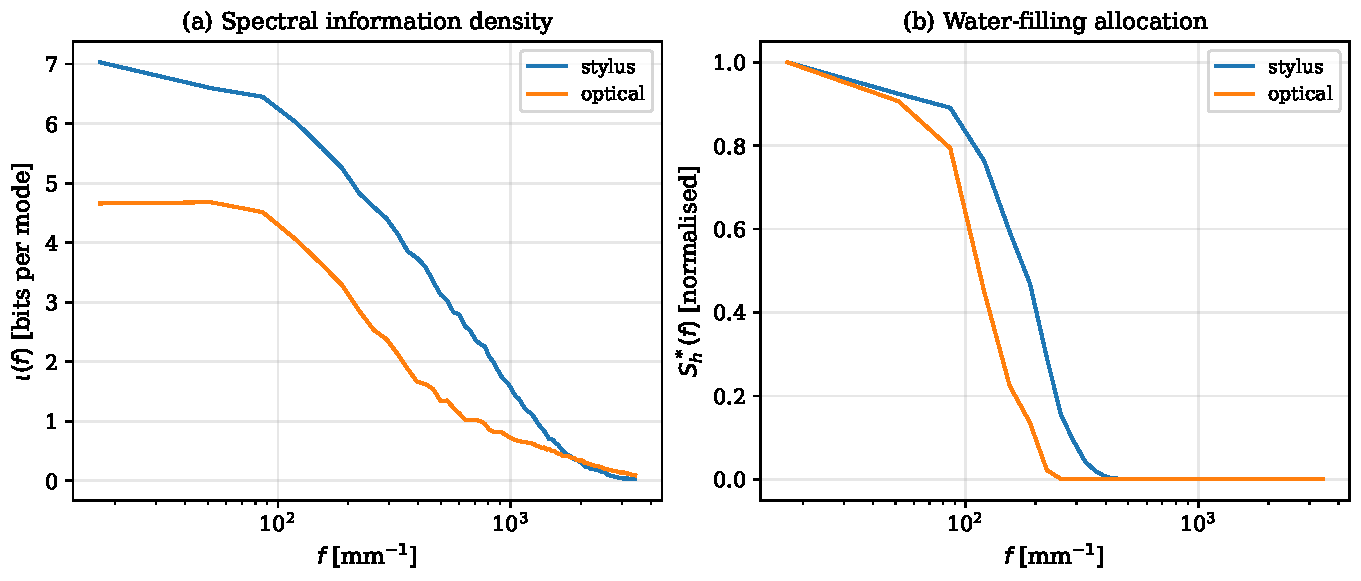
\includegraphics[width=\textwidth]{../pipeline/outputs/iter01/figures/fig7_channel_capacity.pdf}
    \caption{Channel capacity analysis. (a) Spectral information density $\iota(\mathbf{f})$for stylus and optical modalities, showing the information contribution per $ k$-space mode; (b) water-filling power allocation $S_h^*(\mathbf{f})$, identifying the optimal surface spectrum that maximises information throughput given the instrument's transfer function and noise characteristics.}
    \label{fig:capacity}
\end{figure}

\subsection{Fundamental MMSE Reconstruction Limit}

The information-theoretic framework also provides a fundamental lower bound on the mean-square error of any surface reconstruction algorithm. The present analysis assumes a Gaussian channel model (surface heights and measurement noise both Gaussian-distributed), which yields closed-form mutual information and MMSE expressions. For non-Gaussian surface height distributions (e.g., turned, ground, or laser-textured surfaces), these expressions provide a lower bound on mutual information but the exact capacity may differ. Under this Gaussian model, the MMSE is given by~\cite{cover2006elements}:
\begin{equation}
    \mathrm{MMSE} = \sigma^2 - \iint \frac{|H(\mathbf{f})|^2 S_h^2(\mathbf{f})}{|H(\mathbf{f})|^2 S_h(\mathbf{f}) + S_\eta(\mathbf{f})} \, d^2\!f
    \label{eq:mmse}
\end{equation}
This is the surface-metrology analogue of the Shannon lower bound in rate-distortion theory. Under the stated linear Gaussian-channel model (Gaussian surface, Gaussian noise, known $H(\mathbf{f})$ and $S_\eta(\mathbf{f})$), no signal processing algorithm---linear or nonlinear, Bayesian or frequentist---can achieve lower MSE than Eq.~\ref{eq:mmse}; for the nonlinear dilation channel this expression is a linearised benchmark, as noted below.

The reconstructability index $\rho = 1 - \mathrm{MMSE}/\sigma^2$ is mathematically equivalent to the coefficient of determination $R^2$ in regression analysis; its novelty lies in the metrological interpretation---$\rho$ quantifies the fraction of surface variance that is recoverable given a specific instrument's transfer function and noise characteristics---rather than in the formula itself. Because the channel model of Eq.~\ref{eq:channel_model} is linearised, $\rho_\mathrm{stylus}$ is a \emph{linearised} quantity: the true morphological stylus channel is nonlinear, and $\rho$ should be read as a Gaussian-channel benchmark for reconstruction quality rather than an exact MMSE of the dilation channel.

The I-MMSE identity~\cite{guo2005mutual} relates mutual information to reconstruction error (see Supplementary Material \S S4.2 for the derivation). The frequency-resolved Fisher information and its Cram\'er--Rao bound are shown in the Supplementary Material (Fig.~S3).

\subsection{The SNR-Dependent Resolution--Bandwidth Trade-off}

In quantum mechanics, Heisenberg's uncertainty principle states that $\Delta x \cdot \Delta p \geq \hbar/2$. In Fourier analysis, the classical uncertainty principle states that a function and its Fourier transform cannot both be sharply localised: $\Delta x \cdot \Delta f \geq 1/(4\pi)$. Here a \textbf{SNR-Dependent Resolution--Bandwidth Trade-off} is applied to surface measurements, incorporating the finite signal-to-noise ratio of any real instrument (a metrological specialisation of noise-generalised uncertainty bounds from signal processing).

Define the effective spatial resolution $\Delta x_\mathrm{eff}$ as the second-moment width of the instrument's point-spread function and the effective frequency resolution $\Delta f_\mathrm{eff}$as the second-moment width of the noise-truncated transfer function, i.e.\ of the band where $|H(\mathbf{f})|^2 S_h(\mathbf{f}) \geq S_\eta(\mathbf{f})$. With these operational definitions, for a linear measurement operator $\mathcal{M}$with transfer function $ H(\mathbf{f})$ and additive noise $\eta$, the following metrological bound is adopted (its operational definitions, derivation and status are given in Supplementary Material \S S4.3):
\begin{equation}
    \Delta x_\mathrm{eff} \cdot \Delta f_\mathrm{eff} \geq \frac{1}{4\pi}\left(1 + \frac{1}{\overline{\mathrm{SNR}}}\right)
    \label{eq:metrological_uncertainty}
\end{equation}
where $\overline{\mathrm{SNR}} = \iint |H(\mathbf{f})|^2 S_h(\mathbf{f}) \, d^2\!f \,/\, \iint S_\eta(\mathbf{f}) \, d^2\!f$is the area-averaged signal-to-noise ratio. For a perfect, noise-free instrument ($\overline{\mathrm{SNR}} \to \infty$), this reduces to the classical Fourier uncertainty $1/(4\pi)$. For a real instrument, the uncertainty product is \emph{inflated} by the factor $(1 + 1/\overline{\mathrm{SNR}})$.

For the baseline parameters: $\overline{\mathrm{SNR}}_\mathrm{stylus} \approx 56$, $\overline{\mathrm{SNR}}_\mathrm{optical} \approx 32$. The corresponding uncertainty products are:
\begin{itemize}
    \item Stylus: $\Delta x_\mathrm{eff} \cdot \Delta f_\mathrm{eff} \geq 0.081$ (18\% above the classical limit)
    \item Optical: $\Delta x_\mathrm{eff} \cdot \Delta f_\mathrm{eff} \geq 0.083$ (31\% above the classical limit)
\end{itemize}
The stylus approaches the classical Fourier limit more closely than the optical system, despite its lower total information throughput---a manifestation of the trade-off between \emph{information quantity} (throughput) and \emph{information quality} (proximity to fundamental limits). The bound is directly testable and falsifiable: $\Delta x_\mathrm{eff}$ follows from a measured point-spread function, $\Delta f_\mathrm{eff}$ from a measured transfer function, and $\overline{\mathrm{SNR}}$ from measured signal and noise PSDs. A measured product significantly below $(1/4\pi)(1 + 1/\overline{\mathrm{SNR}})$ would falsify the formulation; a product saturating at the bound indicates a well-matched instrument.

\subsection{The Information--Energy--Resolution Trilemma}

For a fixed instrument and measurement area, the mutual information $I$, effective resolution $\Delta x_\mathrm{eff}$, and surface variance $\sigma^2$ are linked by (see Supplementary Material \S S4.3 for derivation):
\begin{equation}
    I \cdot (\Delta x_\mathrm{eff})^2 \approx \sigma^2 \cdot \mathcal{F}(\overline{\mathrm{SNR}})
    \label{eq:trilemma}
\end{equation}
This formalises a three-way trade-off for a fixed instrument and measurement area: the product of extracted information and squared effective resolution is governed by the area-averaged SNR, the single operative lever---surface roughness enters only through $\overline{\mathrm{SNR}}$, since in the explicit form of $\mathcal{F}$ (Supplementary Material \S S4.3) the surface variance cancels. Each element of Eq.~\ref{eq:trilemma} is measurable in principle---$I$ from estimated $H(\mathbf{f})$ and $S_\eta(\mathbf{f})$ via Eq.~\ref{eq:mutual_info}, $\Delta x_\mathrm{eff}$ from the measured PSF, and $\sigma^2$ from the surface PSD---so the relation is experimentally testable rather than purely formal. The dimensionless function $\mathcal{F}(\overline{\mathrm{SNR}})$ is obtained from the water-filling capacity expression combined with the effective resolution definition; its explicit form is given in Supplementary Material \S S4.3.\subsection{The Capacity--Uniformity Product}

The channel capacity $C_\mathrm{total}$ quantifies \emph{how much} information an instrument can transmit. To quantify \emph{how uniformly} it transmits across frequencies, the \textbf{observability condition number} is defined as the ratio of the largest to the smallest power transfer over the measured passband (regularised at the noise floor):
\begin{equation}
    \kappa = \frac{\max_{\mathbf{f}\in\Omega} |H(\mathbf{f})|^2}{\min_{\mathbf{f}\in\Omega} |H(\mathbf{f})|^2}
    \label{eq:gramian}
\end{equation}
where $\Omega$ is the measured $k$-space band and $|H(\mathbf{f})|^2 = H_\mathrm{sensor}(\mathbf{f})$ per Eq.~\ref{eq:transfer_est}. The condition number $\kappa$ measures the disparity between the best-observed and worst-observed $k$-space modes---a perfectly uniform instrument has $\kappa=1$; an instrument that resolves one frequency band 10$\times$ better than another has $\kappa=10$. The \textbf{Capacity--Uniformity Product} is introduced as a practical figure of merit combining throughput and uniformity:
\begin{equation}
    \Xi = \frac{C_\mathrm{total}}{\kappa}
    \label{eq:xi}
\end{equation}
which penalises both low capacity and non-uniform frequency response. For the baseline parameters, $\Xi_o/\Xi_s = 5.9$. Both $C_\mathrm{total}$ and $\kappa$ follow from a calibrated $H(\mathbf{f})$ and $S_\eta(\mathbf{f})$, so $\Xi$ can be evaluated for real instruments from transfer-function calibration measurements (e.g., with binary pseudo-random artefacts~\cite{yashchuk2015binary}).

\subsection{The Research Gap: Why This Framework Is New}

Information theory has been applied to optical imaging since the 1950s. Fellgett~\cite{fellgett1953concerning} and Linfoot~\cite{linfoot1955information} defined the information capacity of an optical system via its OTF. Cox and Sheppard~\cite{cox1986information} extended this to confocal microscopy. In super-resolution fluorescence microscopy, Fisher information analysis has yielded fundamental resolution limits~\cite{ober2004fisher,ram2006framework}. In geophysical inverse problems, information-theoretic criteria guide regularisation parameter selection~\cite{malinverno2004adjustment}.

However, to the best of my knowledge, \textbf{no prior work has systematically applied information theory to the comparison of fundamentally different surface measurement modalities}.\footnote{Search basis: Crossref bibliographic queries (eight targeted keyword sets) and publisher records; the full query log and results are available from the corresponding author upon request. The closest adjacent work found is the resolution and uncertainty literature cited in this section.} The surface metrology literature uses information-theoretic language only metaphorically (``information-rich metrology''~\cite{jiang2007paradigm}) without quantitative Shannon-theoretic content. Three specific gaps motivate the present framework:
\begin{enumerate}
    \item \textbf{The Gaussian-channel mutual information expression}, standard in information theory, has not previously been evaluated to compare profilometry modalities.
    \item \textbf{No channel capacity analysis} has, to the best of my knowledge, been reported for surface metrology instruments, despite the natural interpretation of the profilometer as a communication channel.
    \item \textbf{No fundamental MMSE bound} has, to the best of my knowledge, been established for surface reconstruction from profilometry data, leaving practitioners without a theoretical benchmark against which to compare algorithms.
\end{enumerate}
The framework developed here fills these gaps. Of the diagnostic quantities employed, $\rho$ (reconstructability index) and $\Xi$ (Capacity--Uniformity Product) are, to the best of my knowledge, conceptually new in the surface metrology context. The remaining quantities---$\iota(\mathbf{f})$ (spectral information density), $B_\mathrm{eq}$ (information-equivalent bandwidth: the width of a flat transfer function with the same total information throughput), $\eta$ (information efficiency: the fraction of the noise-free capacity achieved), and $\varepsilon$ (information--energy ratio $I/\sigma^2$)---are standard information-theoretic tools adapted here as convenient diagnostics for profilometry; their definitions follow directly from the Gaussian channel model and are included for completeness. In the notation of Eq.~\ref{eq:mutual_info}, $\eta = I(h;y)/I_\mathrm{perfect}$, where $I_\mathrm{perfect}$ is the mutual information of a noise-free instrument with $H(\mathbf{f})\equiv1$ (regularised at the numerical floor), and $B_\mathrm{eq} = I(h;y)/[\tfrac{1}{2}\log_2(1+\mathrm{SNR}_\mathrm{ref})]$, the area of an ideal flat channel ($H\equiv1$) that transmits the same total information at the reference SNR $\mathrm{SNR}_\mathrm{ref}$.

\subsection{Implications: Toward a More Complete Foundation}

Information-theoretic metrology, as introduced here, differs fundamentally from traditional metrology in its object of study. Traditional metrology asks: ``How accurately does this instrument measure this surface?'' Information-theoretic metrology asks: ``How much information does this instrument extract from this surface, what are the fundamental limits on that extraction, and how efficiently does it convert surface structure into information?''

The shift from accuracy to information has practical consequences:
\begin{itemize}
    \item An instrument with higher RMSE may be \emph{preferable} if it transmits more mutual information about the spatial scales relevant to the application (as the optical system does here for sub-micrometre roughness).
    \item The MMSE bound (Eq.~\ref{eq:mmse}) provides an absolute benchmark: any algorithm claiming to reconstruct a surface from profilometry data can be compared against this limit.
    \item The water-filling solution (see Supplementary Material \S S4.1) suggests an optimal surface spectral shape for instrument testing---calibration artefacts should concentrate their PSD in the $k$-space bands where the instrument's $|H(\mathbf{f})|^2/S_\eta(\mathbf{f})$ is maximal.
    \item The reconstructability index $\rho$ provides a single number (0--1) that is more informative than RMSE for communicating measurement quality to end-users.
\end{itemize}

\subsection*{Practitioner's Summary}

Table~\ref{tab:practitioner} provides a concise reference for practitioners wishing to apply the framework developed in this work.

\begin{table}[htbp]
    \centering
    \caption{Key metrics of the theoretical foundation of surface metrology, their physical meaning, and practical use. Metrics marked $^\dagger$ are standard information-theoretic quantities applied diagnostically to surface metrology; $\rho$ and $\Xi$ are conceptually new in this context.\label{tab:practitioner}}
    \footnotesize
    \setlength{\tabcolsep}{4pt}
    \renewcommand{\arraystretch}{0.95}
    \begin{tabular}{p{2.0cm}p{5.0cm}p{5.0cm}}
        \toprule
        \textbf{Metric} & \textbf{What it tells you} & \textbf{When to use it} \\
        \midrule
        $ I(h;y)$ & Mutual information: total bits revealed about the surface & Interpret at band level; total-throughput ratios are estimator-dependent (Section~\ref{sec:info_theory}) \\[2pt]
        $\iota(\mathbf{f})^\dagger$ & Spectral information density: bits per $ k$-space bin & Identifying which surface scales are measured best \\[2pt]
        $B_\mathrm{eq}^\dagger$ & Information-equivalent bandwidth & Comparing instruments with different transfer functions on a common scale \\[2pt]
        $\eta^\dagger$ & Information efficiency: fraction of ideal capacity achieved & Detecting under-performing instruments \\[2pt]
        $\varepsilon^\dagger = I/\sigma^2$ & Information--energy ratio: bits per unit variance & Normalising comparison across surfaces of different roughness \\[2pt]
        $\rho = 1 - \mathrm{MMSE}/\sigma^2$ & Reconstructability index: recoverable fraction & Communicating quality to end-users ($\rho \to 1$ = near-perfect) \\[2pt]
        $\mathrm{MMSE}$ & Minimum mean-square error: best possible accuracy & Benchmarking algorithms; no algorithm can beat this limit \\[2pt]
        $\kappa$ & Observability condition number: uniformity of response & Detecting instruments with uneven bandwidth \\[2pt]
        $\Xi = C/\kappa$ & Capacity--Uniformity Product: uniformity-weighted capacity & Single-number instrument qualification and purchasing \\[2pt]
        \bottomrule
    \end{tabular}
    \\[4pt]
    {\footnotesize $^\dagger$Standard information-theoretic quantity adapted as a diagnostic for surface metrology; definitions follow directly from the Gaussian channel model (Section~\ref{sec:info_theory}).}
\end{table}

% ============================================================
\section{Conclusions}
% ============================================================

A spectral theory of instrument transfer functions has been presented that explains why stylus and optical profilometry produce different measurements of the same surface, and when they agree. The main findings are:

\begin{enumerate}
    \item The instrument transfer functions $H_\mathrm{stylus}(f_x,f_y)$ and $H_\mathrm{optical}(f_x,f_y)$ are computed from first-principles simulations, and their ratio $R(f_x,f_y)$ identifies modality-dominant $k$-space regions: the stylus dominates below the crossover ($f < f_\mathrm{cross} \approx \SI{454}{mm^{-1}}$); the optical system preserves information to higher frequencies up to its diffraction limit. The empirical stylus transfer is approximately flat with a curvature bias (Eq.~\ref{eq:hstylus}), and the optical model reproduces measured WLI transfer functions from a public dataset (cutoff scale $1.15\pm0.01$). Both modalities exhibit small measurement anisotropy, with the stylus value exceeding the optical value by $\approx 7\times$ ($\alpha_s = 0.0095\pm0.0037$, $\alpha_o = 0.0013\pm0.0006$; ensemble $n=30$).

    \item A $k$-space equivalence regime covering \SI{9.6}{\percent}$\pm$\SI{0.3}{\percent} of the measured bandwidth is identified at $f_\mathrm{cross} = \SI{454}{mm^{-1}}\pm\SI{166}{mm^{-1}}$ ($n=30$), providing a quantitative criterion for when stylus and optical measurements can be considered interchangeable.

    \item The \textbf{reconstructability index} $\rho = 1 - \mathrm{MMSE}/\sigma^2$ --- the recoverable fraction of surface variance under the Gaussian-channel model --- is the most stable metric in the theory for random rough surfaces: the CV is $0.16$ across the Gaussian and ground classes, $0.22$ when the saturating deterministic classes are included, and $0.067$ in the six-class stress test ($n=5$ per class). It saturates at unity for strongly deterministic surfaces, where it is surface-limited rather than instrument-limited.

    \item Extending the theory to scatterometry via the Rayleigh-Rice BSDF-to-PSD relation reveals systematic $ k$-space complementarity: scatterometry probes $\SI{10}{mm^{-1}}$to $\SI{3760}{mm^{-1}}$, extending the measurable bandwidth $\sim$1.9$\times$ beyond the WLI diffraction cutoff ($2\mathrm{NA}/\lambda$) and $\sim$24$\times$ beyond the conventional stylus tip-radius scale ($1/\pi r_\mathrm{tip}$). The three-way comparison indicates that no single modality fully characterises a rough surface across all spatial frequencies; multi-instrument fusion weighted by trust-region $ k$-space complementarity is a practical minimum-variance strategy under the stated independent-noise linear model (see Supplementary Material for a computational demonstration).
\end{enumerate}

These results contribute to the theoretical foundation of surface metrology by connecting measurement instrument physics to principles from communication theory, estimation theory, and vector scattering theory. The instrument transfer functions $H(f)$, the reconstructability index $\rho$, the equivalence regime $\Omega_\mathrm{eq}$, and the three-way $k$-space complementarity of stylus, WLI, and scatterometry provide quantitative tools for instrument selection and inter-comparison. All results are computational. Experimental validation with calibrated artefacts and traceable transfer function measurement~\cite{yashchuk2015binary} remains an open challenge; the predictions and roadmap in~\S\ref{sec:limitations} are offered as falsifiable targets for groups with the necessary laboratory infrastructure. The Complete Physical Framework, scatterometry extension, six-class stress-test, and non-Gaussian ensemble are provided as Supplementary Material.

\section*{Acknowledgements}
The open-source scientific Python ecosystem---NumPy~\cite{harris2020numpy}, SciPy~\cite{virtanen2020scipy}, and Matplotlib~\cite{hunter2007matplotlib}---enabled this computational study. The author declares no competing interests.

\section*{Data Availability}
The simulation code, configuration files, and generated datasets supporting this study will be deposited in a public repository (Zenodo) and cited by DOI upon acceptance; until then they are available from the corresponding author upon reasonable request. An accompanying verification suite (eighteen automated tests) checks the central equations against independent computations, including the stylus transfer-function headline values (T10), the MMSE formula against Monte Carlo Wiener filtering (T11), the parallel-curve ball-standard check (T9) and the information-loss slope (T8). Three committed audit scripts (verification/audit\_scaling\_law.py, verification/audit\_stylus\_channel.py, verification/audit\_mode\_counts.py) regenerate the blocked-validation statistics of the scaling relation, the cross-spectral and coherence analysis of the stylus channel, and the resolved-mode counts. The pipeline is documented in the project README and requirements file. Python 3.9 with NumPy 2.0, SciPy 1.13, and Matplotlib 3.9 was used; all random quantities use fixed seeds (42 for surface generation and the parameter sweep, 123 for the unwrapping-error stream, 100--129 for the 30-member ensemble). The public-data benchmarks use the CC-BY-4.0 datasets of Hirose et al.\ (Zenodo record 10.5281/zenodo.15750880, DOI 10.1364/AO.562002) and Aksulu (ball-standard calibration profiles, Zenodo record 10.5281/zenodo.4471347), fetched by verification/fetch\_public\_data.sh with provenance recorded in data\_public/. A complete snapshot of the repository (code, configurations, figure scripts and generated outputs) is preserved and available from the corresponding author on request; it is prepared for public deposit upon acceptance.

\bibliographystyle{elsarticle-num}
\bibliography{references}

\end{document}
